\ifx\wholebook\relax \else

\documentclass[UTF8]{article}

\usepackage[nomarginpar
  %, margin=.5in
]{geometry}

\addtolength{\oddsidemargin}{-0.05in}
\addtolength{\evensidemargin}{-0.05in}
\addtolength{\textwidth}{0.1in}

\usepackage[cn]{../../prelude}

\setcounter{page}{1}

\begin{document}

\title{参考答案}

\author{刘新宇
\thanks{{\bfseries 刘新宇} \newline
  Email: liuxinyu95@gmail.com \newline}
  }

\maketitle
\fi

\markboth{参考答案}{编程中的数学}

\chapter*{参考答案}
\phantomsection  % so hyperref creates bookmarks
\addcontentsline{toc}{chapter}{参考答案}

\section{前言}

\begin{enumerate}
\item 编程实现一个井字棋游戏是传统人工智能中的经典问题,而计算机可以轻松算出三个数字的和并判断其是否等于15。请利用这个同构编写一个简化的井字棋程序,并做到不被人类玩家击败。

我们的思路是使用《洛书》幻方来同构井字棋游戏,我们用集合$X$, $O$来保存两个玩家所占领的格子。对于前言中的对局,开始时$X = \phi$,$O = \phi$,结束时$X = \{ 2, 5, 7, 1 \}$,$O = \{ 4, 3, 8, 6 \}$。为此我们需要先写一个程序判断一个集合中是否有3个元素相加等于15,从而知道某个玩家获胜与否。

有两种思路解决这个问题,第一种是列举洛书幻方中的所有行、列、对角线,共8个三元组:$\{ \{4, 9, 2\}, \{3, 5, 7\}, ..., \{2, 5, 8\} \}$。然后看是否某个三元组包含在玩家占领的格子集合中。第二种比较有趣,假设玩家占领了格子$ X = \{x_1, x_2, ..., x_n\}$。这些格子按照洛书幻方中的元素升序排列。我们可以先选出$x_1$,然后用左右两个指针$l, r$分别指向下一个元素和最后一个元素,然后把这3个数加起来$s = x_1 + x_l + x_r$,如果等于15,说明玩家连成一条直线已经获胜了。如果小于15,由于元素是升序排列的,我们可以把左侧指针$l$加一,然后再次尝试;如果大于15,我们把右侧指针$r$减一,然后再次尝试。如果左右指针相遇,说明固定$x_1$没有找到相加等于15的三元组,我们选出$x_2$再次进行这样的检查。这样最差情况总共进行$(n - 2)+ (n - 3) + ... + 1$次检查就得知玩家是否获胜了。

\lstset{language=Python
    , frame=single
}
\begin{lstlisting}
def win(s):
    n = len(s)
    if n < 3:
        return False
    s = sorted(s)
    for i in range(n - 2):
        l = i + 1
        r = n - 1
        while l < r:
            total = s[i] + s[l] + s[r]
            if total == 15:
                return True
            elif total < 15:
                l = l + 1
            else:
                r = r - 1
    return False
\end{lstlisting}

这样给定$X$和$O$,就能判断局面。如果$X$和$O$占满全部9个格子,还未分出胜负,则表示平局。接下来我们用传统人工智能中的$min-max$方法来实现井字棋,我们给每个局面一个评分,一方试图让评分最大化,称为正方;另一方试图让评分最小化,称为反方,从而实现对抗。平局的话评分为0,如果某个局面让正方获胜,我们设置评分为10,反方获胜评分为-10。这个分数值完全是随意设置的,不影响结果。

\begin{lstlisting}
WIN = 10
INF = 1000

# Lo Shu magic square
MAGIC_SQUARE = [4, 9, 2,
                3, 5, 7,
                8, 1, 6]

def eval(x, o):
    if win(x):
        return WIN
    if win(o):
        return -WIN
    return 0

def finished(x, o):
    return len(x) + len(o) == 9
\end{lstlisting}

对于任何一个对局,我们都让计算机不断向前探索,直到找到输赢或者平局的确定局面才停下来。探索的方法是穷尽当前所有能占领的格子,然后转换身份,考虑自己是对方时怎样对抗。对于所有候选方案,如果是正方,就选择评分高的方案,如果是反方,就选择评分低的方案。

\begin{lstlisting}
def findbest(x, o, maximize):
    best = -INF if maximize else INF
    move = 0
    for i in MAGIC_SQUARE:
        if (i not in x) and (i not in o):
            if maximize:
                val = minmax([i] + x, o, 0, not maximize)
                if val > best:
                    best = val
                    move = i
            else:
                val = minmax(x, [i] + o, 0, not maximize)
                if val < best:
                    best = val
                    move = i
    return move
\end{lstlisting}

$min-max$是一个递归搜索的过程,为了尽快获胜,我们在评分上加上对向前探索步数的考虑。如果是正方,就从评分中减去递归深度,而对于反方,则加上递归深度。

\begin{lstlisting}
def minmax(x, o, depth, maximize):
    score = eval(x, o)
    if score == WIN:
        return score - depth
    if score == -WIN:
        return score + depth
    if finished(x, o):
        return 0  # draw
    best = -INF if maximize else INF
    for i in MAGIC_SQUARE:
        if (i not in x) and (i not in o):
            if maximize:
                best = max(best, minmax([i] + x, o, depth + 1, not maximize))
            else:
                best = min(best, minmax(x, [i] + o, depth + 1, not maximize))
    return best
\end{lstlisting}

现在我们就做出一个无法被人类击败的程序了,我们的程序在背后用洛书幻方对抗人类玩家:

\begin{lstlisting}
def board(x, o):
    for r in range(3):
        print "-----------"
        for c in range(3):
            p = MAGIC_SQUARE[r*3 + c]
            if p in x:
                print "|X",
            elif p in o:
                print "|O",
            else:
                print "| ",
        print "|"
    print "-----------"

def play():
    x = []
    o = []
    while not (win(x) or win(o) or finished(x, o)):
        board(x, o)
        while True:
            i = int(input("[1..9]==>"))
            if i not in MAGIC_SQUARE or MAGIC_SQUARE[i-1] in x or
               MAGIC_SQUARE[i-1] in o:
                print "invalid move"
            else:
                x = [MAGIC_SQUARE[i-1]] + x
                break
        o = [findbest(x, o, False)] + o
    board(x, o)
\end{lstlisting}

\end{enumerate}

\section{数字}

\begin{enumerate}
\item 定义0的后继为1,证明对于任何自然数都有$a \cdot 1 = a$

首先用数学归纳法证明$0 + a = a$这个结论,见附录\textbf{加法交换律的证明}。然后:
\[
\begin{array}{rlr}
a' \cdot 1 & = a' \cdot 0' & \text{定义0的后继为1} \\
           & = a' \cdot 0 + a' & \text{乘法定义规则二} \\
           & = 0 + a' & \text{乘法定义规则一} \\
           & = a' & \text{此前证明的结论}
\end{array}
\]

\item 证明乘法分配律

可以用数学归纳法证明左侧的分配律$c(a + b) = ca + cb$。首先是$b = 0$的情况:

\bre
c(a + 0) & = & ca & \text{加法规则一} \\
         & = & ca + 0 & \text{反向用加法规则一} \\
         & = & ca + c0 & \text{反向用乘法规则一} \\
\ere

递推假设$c(a + b) = ca + cb$,接下来证明$c(a + b') = ca + cb'$

\bre
c(a + b') & = & c(a + b)' & \text{加法规则二} \\
          & = & c(a + b) + c & \text{乘法规则二} \\
          & = & ca + cb + c & \text{递推假设} \\
          & = & ca + (cb + c) & \text{加法结合律} \\
          & = & ca + cb' & \text{反向用乘法规则二} \\
\ere

\item 证明乘法结合律和交换律

我们只证明乘法结合律$(ab)c = a(bc)$,乘法交换律的证明则给出一个提纲。利用数学归纳法,首先是$c = 0$的情况:

\bre
(ab)0 & = & 0 & \text{乘法规则一} \\
      & = & a0 & \text{反向用乘法规则一} \\
      & = & a(b0) & \text{反向用乘法规则一} \\
\ere

递推假设$(ab)c = a(bc)$,接下来要证明$(ab)c' = a(bc')$

\bre
(ab)c' & = & (ab)c + ab & \text{乘法规则二} \\
       & = & a(bc) + ab & \text{递推假设} \\
       & = & a(bc + b) & \text{上题证明的分配律} \\
       & = & a(bc') & \text{反向用乘法规则二} \\
\ere

证明乘法交换律可以分为三步,都使用数学归纳法。首先证明$1a = a$,然后再证明右侧的分配律$(a + b)c = ac + bc$,最后再证明交换律。

\item 如何利用皮亚诺公里验证3 + 147 = 150

我们先看看经典的2 + 2 = 4是怎么证明的:

\bre
2 + 2 & = & 0'' + 0'' & \text{2是0的两次后继} \\
      & = & (0'' + 0')' & \text{加法定义规则二} \\
      & = & ((0'' + 0)')' & \text{加法定义规则二} \\
      & = & ((0'')')' & \text{加法定义规则一} \\
      & = & 0'''' = 4 & \text{0的4次后继} \\
\ere

显然用这个方法证明3 + 147 = 150的话太冗长了,我们可以用先前证明的加法交换律证明147 + 3 = 150会容易一些。另一个方法是通过数学归纳法证明$3 + a = a'''$。

\item 试给出乘法分配律,乘法结合律,和乘法交换律的几何解释。

\begin{figure}[htbp]
 \centering
 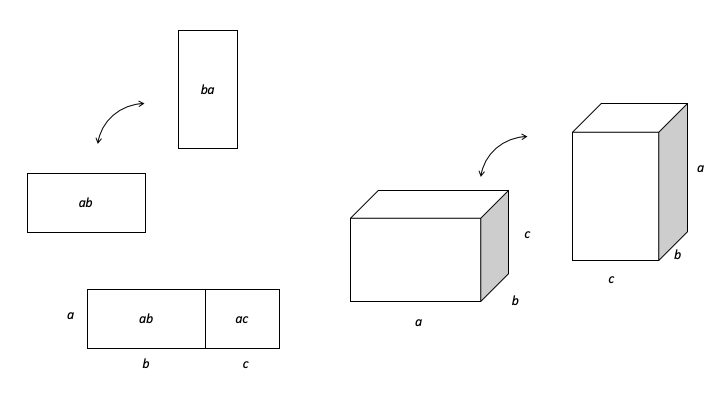
\includegraphics[scale=0.4]{img/geometric-arithmetic.png}
 \captionsetup{labelformat=empty}
 \caption{乘法交换律、结合律、分配律的几何解释}
 \label{fig:geometric-arithmetic}
\end{figure}


\item 使用$foldn$定义平方$()^2$。

可以利用递推关系$(n+1)^2 = n^2 + 2n + 1$来定义平方:

\[
()^2 = 2nd \cdot foldn\ (0, 0)\ h
\]

其中$h$接受一对值$(i, s)$,分别代表自然数$i$和它的平方$s$。它将第一个值递增1,然后利用平方展开式求出下一个平方数。

\[
h\ (i, s) = (i + 1, s + 2i + 1)
\]

\item 使用$foldn$定义$()^m$,计算给定自然数的$m$次幂。

一种简单的方法是借助第一章中定义的$m^{()} = foldn(1, (\cdot m))$来定义$()^m$:

\[
()^m = 2nd \cdot foldn\ (0, 0)\ h
\]

其中

\[
h\ (i, b) = (i + 1, (i + 1)^m)
\]

这看起来有些奇怪,所有中间计算都被直接丢掉了。另一种方法是利用牛顿二项式定理:

\[
(n + 1)^m = n^m + \binom{m}{1} n^{m-1} + ... + \binom{m}{m-1} n + 1
\]

这样就建立了递推关系:

\[
(n)^m = 2nd(foldn\ (1, 1)\ h\ (n - 1))
\]

其中

\[
h (i, x) = (i + 1, C \cdot X)
\]

这里$C \cdot X$是二项式系数和各次幂的点积$C \cdot X = \sum c_j x_j$。各次幂可以通过对$x$不断除以$i$求出,二项式定理的系数可以由帕斯卡三角形逐行递推得到。下面是综合在一起的例子程序:

\lstset{language=Haskell
    , frame=single
}
\begin{lstlisting}
exp m n = snd $ foldn (1, 1) h (n - 1) where
  cs = foldn [1] pascal m
  h (i, x) = (i + 1, sum $ zipWith (*) cs xs) where
    xs = take (m + 1) $ iterate (`div` i) x

pascal = gen [1] where
  gen cs (x:y:xs) = gen ((x + y) : cs) (y:xs)
  gen cs _ = 1 : cs
\end{lstlisting}

\item 使用$foldn$定义奇数的和。它会产生怎样的序列?

用$foldn$定义1 + 3 + 5 + ...为$2nd \cdot foldn\ (1, 0)\ h$,其中:

\[
h\ (i, s) = (i + 2, s + i)
\]

如第一章中习题下的插图所示,奇数和总是平方数。

\item 地面上有一排洞,一只狐狸藏在某个洞中。每天狐狸会移动到相邻的下一个洞里。如果每天只能检查一个洞,请给出一个捉到狐狸的策略,并证明这个策略有效。如果狐狸每天移动的不止一个洞呢?

不管狐狸在哪个洞中,我们只检查奇数洞1, 3, 5, ...必然会捉到狐狸。观察下面的表格

\btab{c|c|c|c|c}
1 & 3 & 5 & ... & 2m - 1 \\
\hline
m & m + 1 & m + 2 & ... & 2m - 1 \\
\etab

狐狸第一天在第$m$个洞中,解方程$m + k = 2k + 1$,得出当$k = m -1$天之后,我们恰好检查第$2m-1$洞,而狐狸恰好也在这个洞中。下面使用$foldn$展示了这一过程:

\[
\begin{array}{l}
fox\ m = foldn\ (1, m)\ h\ (m - 1) \\
\text{其中}: h\ (c, f) = (c + 2, f + 1) \\
\end{array}
\]

如果狐狸第一天在第$p$个洞中,每天移动$q$个洞,我们可以把这样的组合列为$(p, q)$的数偶。然后参考第6章无穷中的方法将其映射到自然数上进行枚举。

\item 表达式$foldr(nil, cons)$定义了什么?

定义了列表本身。

\item 读入一串数字(数字字符串),用$foldr$将其转换成十进制数。如果是16进制怎么处理?如果含有小数点怎么处理?

如果个位在左,高位在右,传入数字列表,则可以这样转换:

\[
foldr\ (c\ d \mapsto 10d + c)\ 0
\]

但如果个位在右,并且列表元素是数字字符,则需要调整为:

\[
1st \cdot foldr\ (c, (d, e) \mapsto ((toInt\ c)e + d, 10e))\ (0, 1)
\]

只要将其中的10换成16,就可以处理16进制。如果传入的字符串含有小数点,只要在遇到小数点时将当前结果$d$除以$e$就可以得到小数部分的值。

\[
1st \cdot foldr\ h\ (0, 1)
\]

其中

\[
h\ (c, (d, e)) = \begin{cases}
c = '.' & (d / e, 1) \\
\text{否则} & ((toFloat\ c)e + d, 10e) \\
\end{cases}
\]

\item 乔恩$\cdot$本特利在《编程珠玑》中给出了一个求最大子序列和的问题。给定整数序列$\{x_1, x_2, ..., x_n\}$,求哪段子序列$i, j$,使得和$x_i + x_{i+1} + ... + x_j$最大。请用$foldr$解决这道题。

如果序列中的元素都是正数,那么最大子序列和必然就是全部元素加到一起。这是因为加法对于正数是单调增加的。如果序列中都是负数,那么最大和就是空序列的和0。对于一个子序列,如果继续加上正数,则和增加,如果加上负数则和减小。我们可以在fold过程中不断维护、更新两个量:一个是已经发现的最大子序列和$S_m$,另一个是到目前检查的元素为止的这一段子序列的和$S$。如果加上下一个元素后$S$超过了$S_m$,表明找到了更大的子序列和。为此我们用$S$替换掉$S_m$;如果加上下一个元素后$S$变成了负数,说明我们完成了上一个子序列的检查,应该开始一段新的子序列检查了。

\blre
max_s & = & 1st \cdot foldr\ f\ (0, 0) \\
\text{其中}: & & f\ x\ (S_m, S) = (S_m', S') \\
& & \text{在$f$中}:  S' = max(0, x + S), S_m' = max(S_m, S') \\
\elre

如果除了最大子序列和,还希望返回子序列,我们可以在fold过程中使用两对值$P_m$和$P$,每对值都包括子序列的和与子序列本身$(S, L)$。

\blre
max_s & = & 1st \cdot foldr\ f\ ((0, []), (0, [])) \\
\text{其中}: & & f\ x\ (P_m, (S, L)) = (P_m', P') \\
& & \text{在$f$中}:  P' = max((0, []), (x + S, x:L)), P_m' = max(P_m, P') \\
\elre

\item 最长无重复字符子串问题。任给一个字符串,求出其中不包含重复字符的最长子串。例如``abcabcbb''的最长无重复字符子串为``abc''。请使用$foldr$求解。

我们给出两种解法。传统的解法是在fold过程中维护一个已发现的最长无重复字符的子串,不断记录并检查遇到的字符$c$上次出现的位置。如果$c$未出现过,或者出现在当前正在检查的子串之前,则延长当前的子串,并和已发现的最长子串比较。否则,说明当前正在检查的子串含有重复字符,需要从上次重复字符出现的位置后开始接下来的检查。

\[
longest(S) = fst2 \cdot foldr\ f\ (0, |S|, |S|, \varnothing)\ zip(\{1, 2, ...\}, S)
\]

其中fold的起始值是一个4元组,含义分别是已经找到的最长子串的长度,最长子串的右侧截止位置,当前正在检查的子串的右侧截止位置,和记录各个不同字符上次出现位置的映射表格。$fst2$能够取出4元组中的前两个作为结果。为了方便在fold过程中得知当前字符的位置,我们将字符串$S$和代表位置的自然数序列$zip$在一起。最关键的函数$f$定义如下:

\[
f\ (i, c)\ (n_{max}, e_{max}, e, Idx) = (n_{max}', e_{max}', e', Idx[c] = i)
\]

其中:

\[ \begin{array}{l}
n_{max}' = max(n_{max}, e' - i + 1) \\
e' = \begin{cases}
  c \notin Idx: & e \\
  Idx[c] = j: & min(e, j - 1) \\
  \end{cases} \\
e_{max}' = \begin{cases}
  e' - i + 1 > n_{max}: & e' \\
  \text{否则}: & e_{max} \\
  \end{cases} \\
\end{array} \]

由于$foldr$是从右侧开始,所以我们使用截止位置。而传统的编程使用起始位置,例如:

\begin{algorithmic}
\Function{Longest}{$S$}
  \State $Idx \gets \varnothing$
  \State $n_{max} \gets 0, s_{max} \gets 0, s \gets 0$
  \For{$i \in \{0, 1, ... |S|\}$}
    \If{$S[i] \in Idx$}
      \State $j \gets Idx[S[i]]$
      \State $s = max(s, j + 1)$
    \EndIf
    \If{$i - s + 1 > n_{max}$}
      \State $s_{max} \gets s$
    \EndIf
    \State $n_{max} \gets max(n_{max}, i - s + 1)$
    \State $Idx[S[i]] = i$
  \EndFor
  \State \Return $S[s_{max} ... s_{max} + n_{max}]$
\EndFunction
\end{algorithmic}

第二种方法是利用素数。我们将每个不同的字符$c$映射到一个素数$p_c$上,对于任何一个字符串$S$,我们可以计算出一个素数的乘积:

\[
P = \displaystyle \prod_{c \in S} p_c
\]

这样,对于任何一个新字符$c'$,我们可以通过其对应的素数$p'$是否整除$P$来判断$c'$是否在$S$中出现过。根据这一点,我们可以设计出一个解法,在fold过程中,不断维护更新子串的的素数积。如果发现一个字符对应的素数可以整除这个积,就说明发现了重复字符。此时,我们截断这个子串中含有重复字符的部分。在这一过程中,我们还要不断更新已发现的最长子串。

\[
longest = fst \cdot foldr\ f\ ((0, []), (0, []), 1)
\]

其中fold的起始值是一个三元组,三元组中的前两个元素是数偶,分别表示已找到的最长子串的长度和内容,当前检查的子串的长度和内容。三元组中最后一个值是素数积,其起始值是1。函数$f$定义为:

\[
f\ c\ (m, (n, C), P) = \begin{cases}
  p_c | P : & update(m, (n + 1, c : C), p_c \times P) \\
  \text{否则}: & update(m, (|C'|, C'), \displaystyle \prod_{x \in C'} p_x) \\
\end{cases}
\]

其中:

\[ \begin{array}{l}
update(a, b, P) = (max(a, b), b, P) \\
C' = c : takeWhile\ (\neq c)\ C \\
\end{array} \]

\item 观察斐波那契的叠加定义,它的后继计算$(m', n') = (n, m + n)$相当于一个矩阵乘法:
\[
\begin{pmatrix} m' \\ n' \end{pmatrix} =
\begin{pmatrix} 0 & 1 \\ 1 & 1 \end{pmatrix}
\begin{pmatrix} m \\ n \end{pmatrix}
\]
起始值是$(0, 1)^T$。这样斐波那契数列就在矩阵乘方下和自然数同构:
\[
\begin{pmatrix}F_n \\ F_{n+1} \end{pmatrix} = \begin{pmatrix} 0 & 1 \\ 1 & 1 \end{pmatrix}^n\begin{pmatrix} 0 \\ 1 \end{pmatrix}
\]
设计一个程序,快速计算2阶方阵的幂。求得斐波那契数列的第$n$个元素。

首先要定义2阶方阵的乘法,以及2阶方阵和向量的乘法:

\[
\begin{pmatrix}
a_{11} & a_{12} \\
a_{21} & a_{22} \\
\end{pmatrix}
\times
\begin{pmatrix}
b_{11} & b_{12} \\
b_{21} & b_{22} \\
\end{pmatrix}
=
\begin{pmatrix}
a_{11} b_{11} + a_{12} b_{21} & a_{11} b_{12} + a_{12} b_{22} \\
a_{21} b_{11} + a_{22} b_{21} & a_{21} b_{12} + a_{22} b_{22} \\
\end{pmatrix}
\]

以及

\[
\begin{pmatrix}
a_{11} & a_{12} \\
a_{21} & a_{22} \\
\end{pmatrix}
\times
\begin{pmatrix}
b_{1} \\
b_{2} \\
\end{pmatrix}
=
\begin{pmatrix}
a_{11} b_{1} + a_{12} b_{2} \\
a_{21} b_{1} + a_{22} b_{2} \\
\end{pmatrix}
\]

当求矩阵的$n$次方$M^n$时,我们不用真的算$n$次乘法。如果$n=4$那么我们可以第一次算出$M^2$,然后再一次算出$(M^2)^2$,只要两次乘法;如果$n = 5$我们可以利用$M^4 \times M$,这样只要算3次乘法。这样我们可以利用$n$的奇偶性,递归地快速计算。

\[
M^n = pow(M, n, I)
\]

其中$I$是2阶方阵$\displaystyle \begin{pmatrix} 1 & 0 \\ 0 & 1\end{pmatrix}$。函数$pow$定义为:

\[
pow(M, n, A) = \begin{cases}
n = 0: & A \\
n\text{是偶数}: & pow(M \times M, \dfrac{n}{2}, A) \\
\text{否则}: & power(M \times M, \lfloor \dfrac{n}{2} \rfloor, M \times A)\\
\end{cases}
\]

事实上,我们可以把$n$表示为二进制数,然后对0、1序列进行fold快速计算出$M^n$。

\end{enumerate}

\section{递归}

\begin{enumerate}
\item 我们给出的欧几里得算法是递归的,请消除递归,只使用循环实现欧几里得算法和扩展欧几里得算法。

由于经典的欧几里得算法是尾递归的,所以可以很方便地转换成循环:

\begin{algorithmic}
\Function{GCM}{$a, b$}
\While{$b \neq 0$}
  \State $a, b \gets b, a \bmod b$
\EndWhile
\State \Return $a$
\EndFunction
\end{algorithmic}

然而扩展欧几里得算法的转换就会比较困难。我们观察三个序列$r, s, t$:

\[\begin{array}{l}
r_0 = a, r_1 = b \\
s_0 = 1, s_1 = 0 \\
t_0 = 0, t_1 = 1 \\
 ...  ... \\
r_{i+1} = r_{i-1} - q_{i} r_{i}, \text{其中}: q_{i} = \lfloor r_{i} / r_{i-1} \rfloor \\
s_{i+1} = s_{i-1} - q_{i} s_{i} \\
t_{i+1} = t_{i-1} - q_{i} t_{i} \\
... ...\\
\end{array}\]

显然,当$r_{k+1} = 0$时,序列终止。并且根据欧几里得算法,我们知道此时:
\[
gcm(a, b) = gcm(r_{k-1}, r_{k}) = gcm(r_k, 0) = r_{k}
\]

更重要的是这一结论,此时如下贝祖等式成立:

\[
gcm(a, b) = r_{k} = a s_{k} + b t_{k}
\]

\begin{proof}
我们用数学归纳法来证明这一结论。首先是0和1的时候,我们有:

\blre
0: & r_0 = a & a s_0 + b t_0 = a \cdot 1 + b \cdot 0 = a \\
1: & r_1 = b & a s_1 + b t_1 = a \cdot 0 + b \cdot 1 = b \\
\elre

接下来是递推假设,若$r_{i-1} = a s_{i-1} + b t_{i-1}$和$r_{i} = a s_{i} + b t_{i}$成立,我们看$i+1$时:

\bre
r_{i+1} & = & r_{i-1} - q_{i} r_{i} & \text{序列定义} \\
       & = & (a s_{i-1} + b t_{i-1}) - q_{i} (a s_{i} + b t_{i}) & \text{递推假设} \\
       & = & a (s_{i-1} - q_{i} s_{i}) + b (t_{i-1} - q_{i} t_{i}) & \text{整理} \\
       & = & a s_{i+1} + b t_{i+1} & \text{序列定义} \\
\ere
因此任何时候,我们的序列都满足贝祖等式。
\end{proof}

这样,就可以得出扩展欧几里得算法的非递归实现了:

\begin{algorithmic}
\Function{Ext-GCM}{$a, b$}
  \State $s', s \gets 0, 1$
  \State $t', t \gets 1, 0$
  \While{$b \neq 0$}
    \State $q, r \gets \lfloor a / b \rfloor, a \bmod b$
    \State $s', s \gets s - q s', s'$
    \State $t', t \gets t - q t', t'$
    \State $a, b \gets b, r$
  \EndWhile
  \State \Return $(a, s, t)$
\EndFunction
\end{algorithmic}

\item 大多数编程环境中的取模运算,要求除数、被除数都是整数。但是线段的长度不一定是整数,请实现一个针对线段的取摸运算。它的效率如何?

想象一下尺规作图,只要能够用圆规截取线段,就可以求模了

\begin{algorithmic}
\Function{mod}{$a, b$}
  \While{$b < a$}
    \State $a \gets a - b$
  \EndWhile
  \State \Return $a$
\EndFunction
\end{algorithmic}

显然这是一个线性效率的运算。为了优化,我们引入一个定理:

\begin{lemma}[递归求余定理] % recursive remainder lemma
如果$r = a \bmod 2b$,那么:
\[
a \bmod b = \begin{cases}
r \leq b: & r \\
r > b: & r - b \\
\end{cases}
\]
\end{lemma}

使用这个定理,我们可以把取模运算加快到$log$级别:

\[
a \bmod b \begin{cases}
a \leq b: & a \\
a - b \leq b: & a - b \\
\text{否则}: & \begin{cases}
  a' \leq b: & a', \text{其中} a' = a \bmod (b + b) \\
  a' > b: & a' - b \\
  \end{cases} \\
\end{cases}
\]

利用斐波那契数列的增长方式,罗伯特$\cdot$弗洛伊德和高德纳将上面方法中的递归消除,用纯循环实现了快速取模运算:

\begin{algorithmic}
\Function{mod}{$a, b$}
  \If{$a < b$}
    \State \Return $a$
  \EndIf
  \State $c \gets b$
  \While{$c \leq a$}
    \State $c, b \gets (b + c, c)$ \Comment{用斐波那契的方式的增大$c$}
  \EndWhile
  \While{$b \neq c$}
    \State $c, b \gets (b, c - b)$ \Comment{再将$c$减小回来}
    \If{$c <= a$}
      \State $a \gets a - c$
    \EndIf
  \EndWhile
  \State \Return $a$
\EndFunction
\end{algorithmic}

\item 我们在证明欧几里得算法正确性的过程中说:“每次都保证余数小于除数。即$b > r_0 > r_1 > r_2 > ... > 0$,但是余数不可能小于零。由于起始值是有限的,故最终算法一定中止。”为什么不会出现,$r_{n}$无限接近于零但不等于零的情况?算法一定会中止么?$a$和$b$是可公度的这一前提保证了什么?

可以利用最小数原理(Well-ordering principle)说明可公度量的欧几里得算法一定终止。最小数原理是自然数所具有的一种基本性质,即任何非空的自然数集中都有最小的自然数。该原理可以推广到整数集、有理数集或实数集的有限非空子集。从可公度的定义出发,我们知道余数序列一定构成有限集。

\item 对于二元线性不定方程$ax + by = c$,若$x_1$、$y_1$和$x_2$、$y_2$为两对整数解。试证明$|x_1 - x_2|$的最小值为$b/gcm(a, b)$,且$|y_1 - y_2|$的最小值为$a/gcm(a, b)$。

令$a, b$的最大公约数$g = gcm(a, b)$。如果$x_0, y_0$是不定方程$ax + by = c$的一组解,则下面给出的也是一组解:

\[
\begin{dcases}
  x = x_0 - k \dfrac{b}{g} \\
  y = y_0 + k \dfrac{a}{g}
\end{dcases}
\]

这一点不难证明:

\blre
ax + by & = & a (x_0 - k \dfrac{b}{g}) + b (y_0 - k \dfrac{a}{g}) \\
        & = & a x_0 + b y_0 - a k \dfrac{b}{g} + b k \dfrac{a}{g} \\
        & = & c - 0 = c
\elre

我们接下来证明,所有不定方程的解都可以表示为这一形式。令$x, y$为不定方程的任意一组解,我们有:$ax + by = c$和$a x_0 + b y_0 = c$。因此:

\[
a (x - x_0) + b (y - y_0) = c - c = 0
\]

两边同时除以$a, b$的最大公约数,得:

\[
\dfrac{a}{g} (x - x_0) + \dfrac{b}{g} (y - y_0) = 0
\]

\[
\dfrac{b}{g} (y - y_0)  = - \dfrac{a}{g} (x - x_0)
\]

注意到,左侧能够被$\dfrac{b}{g}$整除,因此它必然也能整除右侧。但是由于$(\dfrac{a}{g}, \dfrac{b}{g}) = 1$,它们互素,所以必然有$\dfrac{b}{g}$整除$(x - x_0)$,不妨令:

\[
x - x_0 = k \dfrac{b}{g}, \text{对于某个} k \in \pmb{Z}
\]

因此

\[
x = x_0 + k \dfrac{b}{g}
\]

将其代入回上面的等式,得出:

\[
y = y_0 - k \dfrac{a}{g}
\]

这样就证明了所有解都必然是这样的形式。显然,任意两组这样的解,其差最小时$k = 1$,即:$|x_1 - x_2|$的最小值为$b/gcm(a, b)$,且$|y_1 - y_2|$的最小值为$a/gcm(a, b)$。

\item 边长为1的正五边形,对角线的长度是多少?试证明本章插图五角星中的线段AC和AG是不可公度的。使用实数表示,它们的比值是什么?

保罗$\cdot$洛克哈特在《度量》一书中\cite{Lockhart2012}展示了一个漂亮的方法。如图所示,如果把正五边形切成如下的三个小三角形,很容易发现$A$和$B$的全等的,而$C$和它们相似(你能证明这一点么?)。这样,如果正五边形的边长为1,对角线长为$d$,则小三角形的底边为1,而两斜边为$d - 1$。这样根据三角形相似,我们有:

\[
  1 / d = (d - 1) / a
\]

解此一元二次方程得$d = \dfrac{\sqrt{5} + 1}{2}$。对于另一个解$d = \dfrac{\sqrt{5} - 1}{2}$,它比边长短,我们舍去了(这个实际上是小三角形的斜边长)。

本章插图中的AC和AG两条线段,根据上述切分的三个三角形,实际上就是正五边形的对角线和边长。假设它们是可公度的,那么则小三角形的底和斜边就是可公度的。那么在递归的五角星图中,内部的小五边形的边和对角线必然也是可公度的。我们可以无限重复这个过程,不会终止。这样就说明我们的假设不成立,正五边形的边长和对角线是不可公度的。用实数表示这个值约等于0.6180339887498949...

\begin{figure}[htbp]
 \centering
 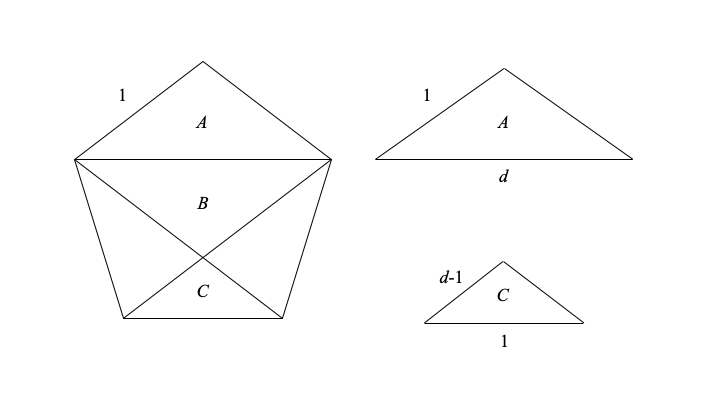
\includegraphics[scale=0.4]{img/pentagram-unit.png}
 \captionsetup{labelformat=empty}
 \caption{边长为1的正五边形}
 \label{fig:pentagram-unit}
\end{figure}

\item 使用$\lambda$变换规则验证$tail\ (cons\ p\ q) = q$。

函数$cons$和$tail$的$\lambda$表达式为:
\[
\begin{array}{rcl}
cons & = & a \mapsto b \mapsto f \mapsto f\ a\ b \\
tail & = & c \mapsto c\ (a \mapsto b \mapsto b)
\end{array}
\]

我们据此来验证$tail\ (cons\ p\ q) = q$这一关系:

\[
\begin{array}{rcl}
tail\ (cons\ p\ q) & = & (c \mapsto c\ (a \mapsto b \mapsto b))\ (cons\ p\ q) \\
                   & \xrightarrow{\beta} & (cons\ p\ q)\ (a \mapsto b \mapsto b) \\
                   & = & ((a \mapsto b \mapsto f \mapsto f\ a\ b)\ p\ q)\ (a \mapsto b \mapsto b) \\
                   & \xrightarrow{\beta} & ((b \mapsto f \mapsto f\ p\ b)\ q)\ (a \mapsto b \mapsto b) \\
                   & \xrightarrow{\beta} & (f \mapsto f \mapsto f\ p\ q)\ (a \mapsto b \mapsto b) \\
                   & \xrightarrow{\beta} & (a \mapsto b \mapsto b)\ p\ q \\
                   & \xrightarrow{\beta} & (b \mapsto b)\ q \\
                   & \xrightarrow{\beta} & q
\end{array}
\]

\item 可以仅仅使用$\lambda$演算来定义自然数。下面是丘奇数的定义:
\[
\begin{array}{r@{\quad:\quad}l}
0 & \lambda f . \lambda x . x \\
1 & \lambda f . \lambda x . f\ x \\
2 & \lambda f . \lambda x . f\ (f\ x) \\
3 & \lambda f . \lambda x . f\ (f\ (f\ x)) \\
  & ...
\end{array}
\]
请利用第一章介绍的内容,定义丘奇数的加法和乘法。

自然数$n$的丘奇数含义是将函数$f$向$x$应用$n$次。我们先定义后继函数:

\[
succ = \lambda n . \lambda f . \lambda x . f\ (n\ f\ x)
\]

其含义是;$f^{n+1}(x)) = f(f^n(x))$。然后定义自然数加法为:

\[
plus = \lambda m . \lambda n . \lambda f . \lambda x . m\ f\ (n\ f\ x)
\]

其含义是:$f^{m + n}(x) = f^m(f^n(x))$。乘法定义为:

\[
mul = \lambda m . \lambda n . \lambda f . \lambda x . m\ (n\ f)\ x
\]

其含义为:$f^{m n} = (f^n)^m(x)$。

\item 以下是丘奇布尔值的定义,以及逻辑运算的一种实现:
\[
\begin{array}{r@{\quad:\quad}l}
\textbf{true} & \lambda x . \lambda y . x \\
\textbf{false} & \lambda x . \lambda y . y \\
\textbf{and} & \lambda p . \lambda q . p\ q\ p \\
\textbf{or} & \lambda p . \lambda q . p\ p\ q \\
\textbf{not} & \lambda p . p\ \textbf{false}\ \textbf{true}
\end{array}
\]
其中\textbf{false}的定义和丘奇数0的定义本质上是相同的。试用$\lambda$变换证明:\textbf{and}\ \textbf{true}\ \textbf{false} = \textbf{false};你能给出if...then...else...语句的$\lambda$定义么?

\blre
and\ true\ false & = & (\lambda p . \lambda q . p\ q\ p)\ true\ false \\
 & \xrightarrow{\beta} & true\ false\ true \\
 & = & (\lambda x . \lambda y . x)\ false\ true \\
 & \xrightarrow{\beta} & false \\
\elre

if ... then ... else ...语句的定义:$\lambda p . \lambda a . \lambda b . p\ a\ b$

\item 不用抽象的叠加操作$foldt$,通过递归定义二叉树的逐一映射$mapt$;

\[ \begin{cases}
mapt(f, nil) & = nil \\
mapt(f, node(l, x, r)) & = node(mapt(f, l), f(x), mapt(f, r)) \\
\end{cases}\]

\item 定义一个函数$depth$,计算一棵二叉树的最大深度;

\[
depth = foldt(one, x, y \mapsto 1 + max(x, y), 0)
\]

其中$one$为常函数,总返回1:$one = x \mapsto 1$。

\item 有人认为,二叉树的抽象叠加操作$foldt$应该这样定义:
\[
\begin{array}{l}
foldt(f, g, c, nil) = c \\
foldt(f, g, c, node(l, x, r)) = foldt(f, g, g(foldt(f, g, c, l), f(x)), r)
\end{array}
\]
也就是说,$g : (B \times B) \to B$是一个类似于加法这样的二元函数。能否利用这个$foldt$定义逐一映射$mapt$?

无法用这样的$foldt$定义逐一映射。一棵树被逐一映射后仍然是一棵结构一样的树,只是树中的元素被映射到其它值上。注意$f$的类型:$f : A \to B$,它将一棵树中的类型为$A$的元素映射为类型$B$。而函数$g$的类型为$g : (B \times B) \to B$,它只能对类型为$B$的值进行映射,却无法保持树的结构。

\item 排序二叉树(又称二叉搜索树)是一种特殊的二叉树,如果二叉树的元素类型A是可比较的,并且对任何非空节点$node(l, k, r)$都满足:左子树$l$中的任何元素都小于$k$,右子树$r$中的任何元素都大于$k$。定义二叉树的插入函数$insert(x, t) : (A \times Tree\ A) \to Tree\ A$

\[ \begin{cases}
insert(x, nil) = node(nil, x, nil) \\
insert(x, node(l, k, r)) = \begin{cases}
  x < k: & node(insert(x, l), k, r) \\
  \text{否则}: & node(l, k, insert(x, r)) \\
\end{cases} \\
\end{cases}\]

\item 为多叉树定义逐一映射。能否利用多叉树的叠加操作来定义?如果不能,应当怎样修改叠加操作?

和上题类似,我们需要修改多叉树的叠加操作,来保持树的结构:

\[
\begin{cases}
foldm(f, g, c, nil) & = c \\
foldm(f, g, c, node(x, ts)) & = g(f(x), map(foldm(f, g, c), ts)) \\
\end{cases}
\]

其中$map$是列表的逐一映射函数。然后就可以利用这一叠加操作定义逐一映射:

\[
mapm(f) = foldm(f, node, nil)
\]

\end{enumerate}

\section{对称}

\begin{enumerate}
\item 全体偶数在加法下是否构成一个群?

的确构成一个群。偶数加偶数仍然是偶数,加法本身是可结合的。单位元是0,逆元是相反数。

\item 能否找到一个整数的子集,使得它在整数乘法下构成一个群?

子集$\{ -1, 1 \}$在乘法下构成一个群。单位元是1。每个元素都是自己的逆元。

\item 所有正实数在乘法下是否构成一个群?

是的。正实数在乘法下封闭,乘法本身具备结合性。单位元是1,任何元素的逆元是其倒数。

\item 整数在减法下是否构成一个群?

不构成群。这是因为减法不具备结合性。例如:(3 - 2) - 1 = 0,但3 - (2 - 1) = 2。

\item 举一个只有两个元素的群的例子。

前面题目中的${-1, 1}$在加法下构成群。另外一个例子是布尔值$\{T, F\}$,在逻辑异或xor下构成一个群。异或是封闭的,并且具备结合性。单位元是F。任何元素和F异或的结果是其本身。任何元素的逆元则是其本身。

\item 魔方群的单位元是什么?$F$的逆元是什么?

魔方群的单位元是恒等变换。这一变换将任何魔方状态变回它本身(维持不变)。$F$的逆元是$F'$,即正面逆时针转90度。

\item 布尔值构成的集合\{True, False\},在“逻辑或”运算$\lor$下构成一个幺半群。称为任意(Any)逻辑幺半群。它的单位元是什么?

False

\item 布尔值构成的集合\{True, False\},在“逻辑与”运算$\land$下构成一个幺半群。称为全部(All)逻辑幺半群。它的单位元是什么?

True

\item 对可比类型的元素进行比较时,会有三种结果,我们把它们抽象为$\{<, =, >\}$,针对这个集合,定义一个二元运算使得它们构成一个幺半群。这个幺半群的单位元是什么?

定义二元运算:

\blre
< \circ\ x & = & < \\
= \circ\ x & = & x \\
> \circ\ x & = & > \\
\elre

其中$x$是三种元素中的任一个。则这三种序关系构成一个幺半群。单位元是$=$。

\item 证明群、幺半群、半群的幂满足交换律:$x^mx^n = x^nx^m$

为了证明交换律,我们先证明一个\textbf{预备结论}:$x^n x = x x^n$。使用数学归纳法。对于群和幺半群,首先是$n = 0$时的情形:

\[
x^0 x = e x = x = x e = x x^0
\]

对于半群由于没有单位元,我们考虑$n = 1$时的情形:

\[
x^1 x = x x = x x^1
\]

接下来假设$n$时结论成立,即:$x^n x = x x^n$,现在考虑$n + 1$时:

\bre
x^{n + 1} x & = & (x x^n) x & \text{幂的递归定义} \\
  & = & x (x^n x) & \text{结合性} \\
  & = & x (x x^n) & \text{递归假设} \\
  & = & x x^{n + 1} & \text{幂的递归定义} \\
\ere

利用这个结论,接下来我们使用数学归纳法,证明幂的交换性。对于群和幺半群,先验证$n = 0$时的情况:

\bre
x^m x ^ 0 & = & x^m e & \text{0次幂的定义} \\
  & = & x^m & \text{单位元的定义} \\
  & = & e x^m & \text{单位元的定义} \\
  & = & x^0 x^m & \text{0次幂的定义} \\
\ere

对于半群,由于没有单位元,我们验证$n = 1$时的情况:

\bre
x^m x ^ 1 & = & x^m x & \text{1次幂的定义} \\
  & = & x x^m & \text{此前证明的结论} \\
  & = & x^1 x^m & \text{1次幂的定义} \\
\ere

假设$n$时,幂的交换律成立:$x^mx^n = x^nx^m$,则$n+1$时:

\bre
x^m x^{n+1} & = & x^m (x x^n) & \text{幂的递归定义} \\
  & = & (x^m x) x^n & \text{乘法结合律} \\
  & = & x x^m x^n & \text{此前证明的结论} \\
  & = & x (x^m x^n) & \text{乘法结合律} \\
  & = & x (x^n x^m) & \text{递推假设} \\
  & = & (x x^n) x^m & \text{乘法结合律} \\
  & = & x^{n+1} x^m & \text{幂的递归定义} \\
\ere

\item 奇偶判断函数在整数加群$(\pmb{Z},+)$和布尔逻辑与群$(Bool, \land)$下是否构成同态?去除0元素的整数乘法群呢?

为了判断是否构成同态,我们需要检查两点:1、是否是满射;2、是否满足$f(a) f (b) = f(a \cdot b)$。奇偶判断函数虽然是满射,但我们有下面的反例:

$a, b$都是奇数:$odd(a) = odd(b) = True$,它们的和是偶数,故而:$odd(a + b) = False$。而逻辑与的结果:$odd(a) \land odd(b) = True \neq odd(a + b) = False$。

因而不构成同态。

而去除0后的整数乘法群在奇偶判断函数下与逻辑与群构成同态。我们可以验证全部的三种情况:

  \begin{itemize}
  \item $a, b$都是奇数:$odd(a) = odd(b) = True$, 积$ab$仍然是奇数:$odd(ab) = True$。所以$odd(a) \land odd(b) = odd(ab)$;
  \item $a, b$都是偶数:$odd(a) = odd(b) = False$, 积$ab$仍然是偶数:$odd(ab) = False$。所以$odd(a) \land odd(b) = odd(ab)$;
  \item $a, b$一奇一偶:不妨令$odd(a) = True, odd(b) = False$, 积$ab$是偶数:$odd(ab) = False$。所以$odd(a) \land odd(b) = odd(ab)$。
  \end{itemize}

故而是构成同态。

\item 假定两个群$G$和$G'$在映射下同态,群$G$中的元$a \to a'$,那么$a$和$a'$的阶是否相同?

它们的阶相同。我们可以证明这一点。令单位元$e$的像是$e'$,同态映射为$f$。记$a$的阶为$n$,我们有$a^n = e$。

一方面我们有:
\[
f(a^n) = f(e) = e'
\]

另一方面,根据同态的定义,我们有:

\bre
f(a^n) & = & f(a) f(a) ... f(a) & \text{共$n$个} \\
  & = & a' a' ... a' & \text{共$n$个} \\
  & = & (a')^n
\ere

综合上述两个结果,我们有$(a')^n = e'$。所以$a$和$a'$的阶相同。

\item 证明一个变换群的单位元一定是恒等变换。

假设某一变换$\epsilon': a \to a^{\epsilon'} = \epsilon'(a)$是变换群的单位元。根据单位元的性质,我们有$\epsilon' \tau = \tau$。即:

\[
\begin{array}{l}
\tau: a \to a^\tau \\
\epsilon' \tau: a \to (a^{\epsilon'})^\tau \\
\end{array}
\]

故而:$a^{\epsilon'} = a = \epsilon'(a)$,也就是$\epsilon'$为恒等变换。

\item 列出$S_4$的全体元素。

(1);

(12), (34), (13), (24), (14), (23);

(123), (132), (134), (143), (124), (142), (234), (243);

(1234), (1243), (1324), (1342), (1423), (1432);

(12)(34), (13)(24), (14)(23)。

共$4!=24$个元素。

\item 将$S_3$的所有元写成不相连的循环置换的乘积。

\btab{c|c|c|c|c|c|c}
排列 & 123 & 213  & 132  & 321  & 231   &  312\\
\hline
置换 & (1) & (12) & (23) & (13) & (123) & (132)\\
\etab

\item 编程将$k$-循环的乘积转换回置换。

\begin{algorithmic}
\Function{Permute}{$C, n$}
  \State $\pi \gets [1, 2, ..., n]$
  \For{$c \in C$}
    \State $j \gets c[1]$
    \State $m \gets |c|$
    \For{$i \gets 2$ to $m$}
      \State $\pi[j] \gets c[i]$
      \State $j \gets c[i]$
    \EndFor
    \State $\pi[c[m]] \gets c[1]$
  \EndFor
  \State \Return $\pi$
\EndFunction
\end{algorithmic}

\item 对称群$S_4$描述了什么几何形状的哪些对称性?

它描述了正四面体(像一个三角粽子)的对称性。正四面体每个顶点有一条对称轴,每个轴上有120度和240度两个旋转对称。穿过相对的两条边有3条对称轴每个轴上有一个翻转对称。再加上恒等变换,一共有$2 \times 4 + 3 + 1 = 12$种对称性。恰好对应对称群$S_4$种的每个元素。

\begin{figure}[htbp]
 \centering
 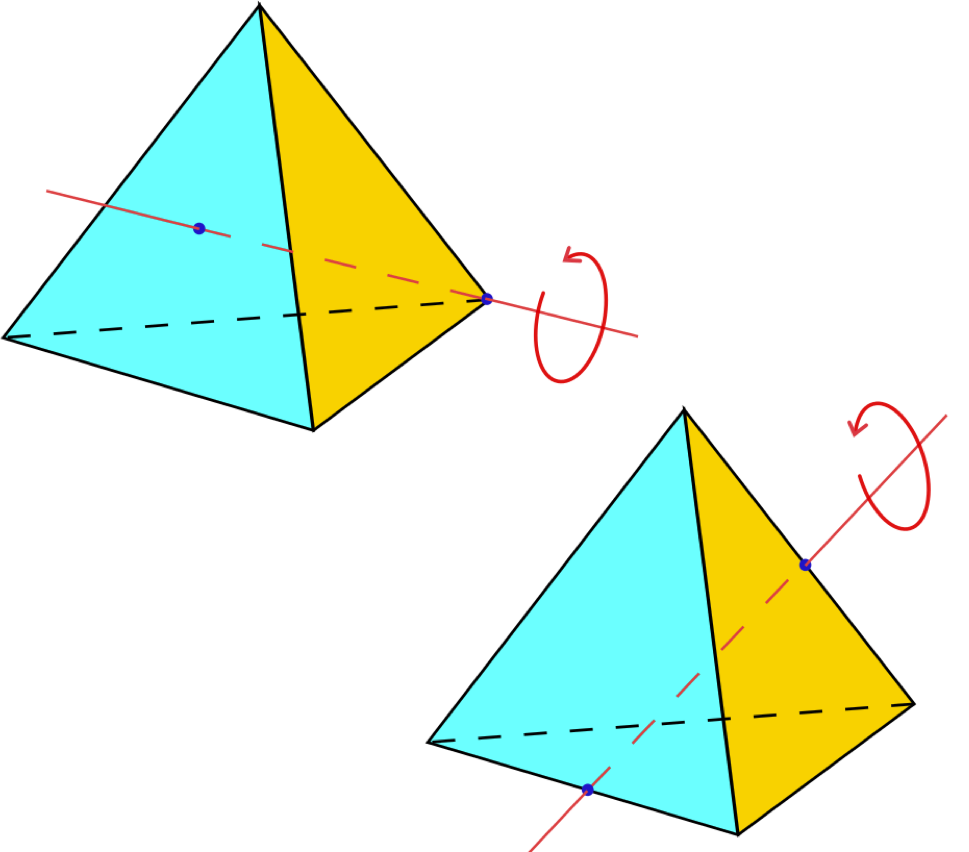
\includegraphics[scale=0.5]{img/tetrahedron.png}
 %\captionsetup{labelformat=empty}
 \caption{正四面体的两种对称轴}
 \label{fig:tetrahedron}
\end{figure}

\item 证明循环群一定是阿贝尔群。

令生成元为$a$,循环群中的任意两个元素可表示为$a$的幂$a^p, a^q$。我们有:
\[
a^p a^q = a^{p + q} = a^{q + p} = a^q a^p
\]
故而循环群一定是阿贝尔群。

\item 证明子群的判定定理。一个群$G$的非空子集$H$构成子群的充分必要条件是:
  \begin{enumerate}[i]
  \item 若$a, b \in H$,有$ab \in H$,
  \item 且任意元素$a \in H$,有$a^{-1} \in H$。
  \end{enumerate}

先证明充分性。条件i保证了$H$对乘法的封闭性,乘法的结合性在$G$中成立,所以在$H$中也成立。因为$H$不空,所以至少存在一个元$a$,根据ii,对应的$a^{-1}$也在$H$中,并且由i,有$aa^{-1} = e \in H$。因此$H$是子群。

反过来在证明必要性。若$H$是一个子群,则i显然成立。对于ii,因为$H$是群,故存在单位元$e'$,在$H$中任取一个元素$a$,有$e'a = a$。因为$e'$和$a$都属于$G$,所以$e'$是方程$ya = a$在$G$中的一个解。但这个方程在$G$中只有一个解,就是$G$的单位元$e$所以$e' = e \in H$。

因为$H$是一个群,所以方程$ya = e$在$H$中存在解$a'$,但$a'$也是这个方程在$G$中的解,而这个方程在$G$中只有一个解,就是$a^{-1}$。所以$a' = a^{-1} \in H$。

\item 列出下图中$H$的左陪集。

\begin{figure*}[htbp]
\centering
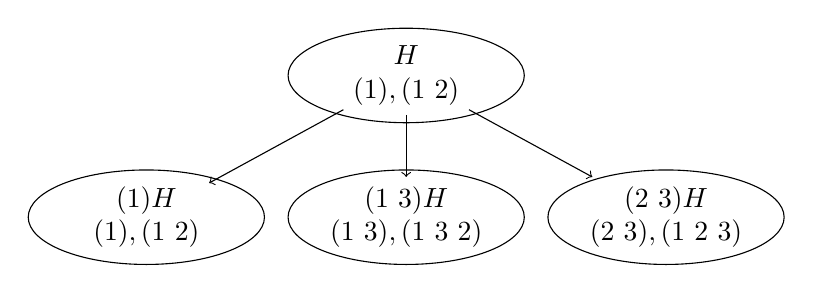
\begin{tikzpicture}[scale=0.6]
\draw (0, 3) circle[x radius=2.5cm, y radius=1cm] node[align=center] (H) {$H$ \\ $(1), (1\ 2)$}
      (-5.5, 0) circle[x radius=2.5cm, y radius=1cm] node[align=center] (H1) {$(1) H$ \\ $(1), (1\ 2)$}
      (0, 0) circle[x radius=2.5cm, y radius=1cm] node[align=center] (H13) {$(1\ 3) H$ \\ $(1\ 3), (1\ 3\ 2)$}
      (5.5, 0) circle[x radius=2.5cm, y radius=1cm] node[align=center] (H23) {$(2\ 3) H$ \\ $(2\ 3), (1\ 2\ 3)$};
\draw[->] (H) edge (H1)
          (H) edge (H13)
          (H) edge (H23);
\end{tikzpicture}
\end{figure*}

用(1), (1 3), (2 3)分别左乘子群$H = \{(1), (1\ 2)\}$得:

\blre
(1) H & = & \{(1), (1\ 2)\} \\
(1\ 3) H & = & \{(1\ 3), (1\ 3\ 2)\} \\
(2\ 3) H & = & \{(2\ 3), (1\ 2\ 3)\} \\
\elre

\item 今天是星期日,$2^{100}$天以后是星期几?

一周有7天,根据费马小定理,$2^{7-1} \equiv 1 \mod 7$。所以:

\blre
2^{100} = 2^{16 \times 6 + 4} & \equiv & 1 \times 2^4 \mod 7 \\
  & \equiv & 16 \mod 7 \\
  & \equiv & 2 \mod 7 \\
\elre

所以是星期二。

\item 任给两个串(字符串或者列表),如何通过编程判断它们可以连成相同的项链?

任给两个长度相同的串$S_1, S_2$,我们可以把$S_1$复制一份接在自己后面,然后检查$S_2$是否是$S_1S_1$的子串。如果是,那么它们可以连成相同的项链。

\[
eqiv(S_1, S_2) = S_2 \subset (S_1 \doubleplus S_1)
\]

\lstset{language=Python, frame=single}
\begin{lstlisting}
def eqiv(s1, s2):
    return (s1 + s1).find(s2) != -1
\end{lstlisting}

\item 编程实现埃拉托斯特尼筛法。

从2开始对于所有的自然数,取出下一个作为素数,然后去掉所有它的倍数,并递归进行这一操作。如下面的Haskell例子程序:
\lstset{language=Haskell}
\begin{lstlisting}
primes = sieve [2..] where
    sieve (x:xs) = x : sieve [y | y <- xs, y `mod` x > 0]
\end{lstlisting}

下面分别是Python和Java的例子程序:
\lstset{language=Python}
\begin{lstlisting}
def odds():
    i = 3
    while True:
        yield i
        i = i + 2

class prime_filter(object):
    def __init__(self, p):
        self.p = p
        self.curr = p

    def __call__(self, x):
        while x > self.curr:
            self.curr += self.p
        return self.curr != x

def sieve():
    yield 2
    iter = odds()
    while True:
        p = next(iter)
        yield p
        iter = filter(prime_filter(p), iter)

list(islice(sieve(), 100))
\end{lstlisting}

\lstset{language=Java}
\begin{lstlisting}
public class Prime {
    private static LongPredicate sieves = x -> true; // initialize sieve as id
    public final static long[] PRIMES = LongStream
        .iterate(2, i -> i + 1)
        .filter(i -> sieves.test(i))
        .peek(i -> sieves = sieves.and(v -> v % i != 0)) // update, chain the sieve
        .limit(100)                 // take first 100
        .toArray();
}
\end{lstlisting}

\item 利用埃拉托斯特尼筛法的思想,编程产生2到100内正整数的欧拉$\upphi$函数表。

我们一边用埃拉托斯特尼筛法产生$n$以内的素数,一边用每个新找到的素数更新一个欧拉$\upphi$函数表。这个函数表被全部初始化为1。对于每个素数$p$,其对应的$\upphi(p) = p(1 - \dfrac{1}{p}) = p - 1$,我们需要把所有$p$的倍数都乘以这个值。但仅仅这样还不够,这是因为$\upphi(p^2) = p^2(1 - \dfrac{1}{p}) = p \upphi(p)$。所以我们接下来要把所有$p^2$倍数的欧拉函数值都乘以$p$,重复这一步骤,再把所有$p^3$倍数的欧拉函数值乘以$p$。继续持续这一过程,直到我们发现$p^m$超过$n$。下面是利用这一思想的解法:

\begin{algorithmic}
\Function{Euler-Totient}{$n$}
  \State $\upphi \gets \{1, 1, ..., 1\}$ \Comment{1到$n$}
  \State $P \gets \{2, 3, ..., n\}$ \Comment{素数筛法序列}
  \While{$P \neq \varnothing$}
    \State $p \gets P[0]$
    \State $P \gets \{x | x \in P, x \bmod p \neq 0\}$
    \State $p' \gets p$
    \Repeat
      \For{$i \gets$ from $p'$ to $n$ step $p'$}
        \If{$p' = p$}
          \State $\upphi[i] \gets \upphi[i] \times (p - 1)$
        \Else
          \State $\upphi[i] \gets \upphi[i] \times p$
        \EndIf
      \EndFor
      \State $p' \gets p' \times p$
    \Until{$p' > n$}
  \EndWhile
  \State \Return $\upphi$
\EndFunction
\end{algorithmic}

\item 编程实现模乘的幂运算,并实现费马素数检测。

我们的思路是参考快速幂的思路,实现模乘的幂运算。
\[
x^y =
\begin{cases}
y \text{是偶数}: & x^{\lfloor y / 2 \rfloor} \\
y \text{是奇数}: & x \cdot x^{\lfloor y / 2 \rfloor} \\
\end{cases}
\]

只要在此基础上,将乘法改为模乘即可:

\begin{algorithmic}
\Function{Mod-Exp}{$x, y, n$}
  \If{$y = 0$}
    \State \Return 1
  \EndIf
  \State $z \gets$ \Call{Mod-Exp}{$x, \lfloor y /2 \rfloor, n$}
  \If{$y$是偶数}
    \State \Return $z^2 \bmod n$
  \Else
    \State \Return $x \cdot z^2 \bmod n$
  \EndIf
\EndFunction
\end{algorithmic}

然后我们利用费马小定理,选取若干“证人”,进行素数检测:

\begin{algorithmic}
\Function{primality}{$n$}
  \State 随机选择$k$个正整数$a_1, a_2, ..., a_k < n$
  \If{$a_i^{n-1} \equiv 1 \mod n$,对于全部$i = 1, 2, ..., k$}
    \State \Return 素数
  \Else
    \State \Return 合数
  \EndIf
\EndFunction
\end{algorithmic}

\item {证明本节的定理,一个没有零因子的环里,两个消去律成立。}

\begin{proof}
假定环$R$没有零因子。因为:
\[
  ab = ac \Rightarrow a(b - c) = 0
\]

在此假定之下,

\[
  a \neq 0, ab = ac \Rightarrow b - c = 0 \Rightarrow b = c
\]

同样可证,

\[
  a \neq 0, ba = ca \Rightarrow b = c
\]

这样$R$里两个消去律都成立。反过来,假定环$R$里第一个消去律成立。因为

\[
  ab = 0 \Rightarrow ab = a0
\]

在此假定之下,

\[
  a \neq 0, ab = 0 \Rightarrow b = 0
\]

这就是说,$R$没有零因子。第二个消去律成立的事后,同样可证。
\end{proof}

\item {证明所有形如$a + b \sqrt{2}$,其中$a, b$是整数的实数对于普通加法和乘法构成一个整环。}

\begin{proof}
我们依次验证三点:

  \begin{enumerate}[i]
  \item 乘法交换律成立
    \bre
      (a + b \sqrt{2})(c + d \sqrt{2}) & = & ac + 2bd + (ad + bc)\sqrt{2} \\
        & = & (c + d \sqrt{2})(a + b \sqrt{2})
    \ere
  \item 有乘法单位元1
    \[
      1 (a + b \sqrt{2}) = (a + b \sqrt{2}) 1 = a + b \sqrt{2}
    \]
  \item 没有零因子
    \[
    (a + b \sqrt{2})(c + d \sqrt{2}) = 0 \Rightarrow a = b = 0 \text{或} c = d = 0
    \]
  \end{enumerate}
\end{proof}

\item {证明$Q[a, b] = Q[a][b]$,其中$Q[a, b]$是所有由$a, b$组成的表达式如$2ab, a + a^2b$等。}

证明之前,我们先举个例子:

\[
 Q[\sqrt{2}, \sqrt{3}] = \{a + b \sqrt{2} + c \sqrt{3} + d \sqrt{6}, \text{其中} a, b, c, d \in Q\}
\]

\bre
Q[\sqrt{2}][\sqrt{3}] & = & \{a + b \sqrt{3}, \text{其中} a, b \in Q[\sqrt{2}]\} \\
  & = & \{a' + b' \sqrt{2} + (c + d \sqrt{2}) \sqrt{3}, \text{其中} a', b', c, d \in Q\} \\
  & = & \{a' + (b' + d) \sqrt{2} + c \sqrt{3} + d \sqrt{6}, \text{其中} a', b', c, d \in Q\}
\ere

\begin{proof}
\[
Q[a][b] = \{x_0 + x_1 b + x_2 b^2 + ... + x_n b^n, \text{其中} x_i \in Q[a]\}
\]
$n$是使得存在多项式$p(b) = 0$的最小整数。现在我们把$x_i$替换成域$Q[a]$的表达式

\bre
Q[a][b] & = & \{ y_{0,0} + y_{0,1} a + y_{0,2} a^2 + ... + y_{0,m} a^m + \\
        &   &   (y_{1,0} + y_{1,1} a + y_{1,2} a^2 + ... + y_{1,m} a^m) b + \\
        &   &   (y_{n,0} + y_{n,1} a + y_{n,2} a^2 + ... + y_{n,m} a^m) b^n \}
\ere

其中,$y_{i,j} \in Q$,整数$m$是使得存在多项式$p(a) = 0$的最小整数。

不失一般性,我们可以认为$m < n$(否则,我们只需令$m' = min(m, n), n' = max(m, n)$),可以进一步整理成:

\bre
Q[a][b] & = & \{ y_{0,0} + y_{0,1} a + y_{1,0} b + y_{0,2} a^2 + y_{1,1} ab + y_{2,0} b^2 + ... \\
        &   &    + y_{0,m} a^m + y_{1,m-1} a^{m-1} b + ... + y_{m, 0} b^m + \\
        &   &    + y_{1,m} a^m b + y_{2, m-1} a^{m-1} b^2 + ... + y_{m, 1} b^{m+1} + ... \\
        &   &    + y_{n, m} a^m b^n \}
\ere

可以看到,这的确是由$a, b$组成的所有表达式构成的域。
\end{proof}

\item {试证明:对于有理数系数的任何多项式$p(x)$,若$E/Q$是扩域,$f$是$E$上的$Q$-自同构,则有$f(p(x)) = p(f(x))$。}

\begin{proof}
由$f$是自同构的定义,我们有:
\[
f(x + y) = f(x) + f(y), f(ax) = f(a) f(x), f(1/x) = 1 / f(x)
\]
并且由于$f$是$Q-$自同构,我们有:
\[
 f(x) = x, \forall x \in Q
\]

令$p(x) = a_0 + a_1 x + ... + a_n x^n$,其中$a_i \in Q$。我们有:

\bre
f(p(x)) & = & f(a_0 + a_1 x + ... + a_n x^n) \\
  & = & f(a_0) + f(a_1 x) + ... + f(a_n x^n) & f(x + y) = f(x) + f(y) \\
  & = & f(a_0) + f(a_1) f(x) + f(a_2) f(x)^2 + ... + f(a_n) f(x)^n & f(ax) = f(a) f(x) \\
  & = & a_0 + a_1 f(x) + a_2 f(x)^2 + ... + a_n f(x)^n & f(x) = x, \forall x \in Q \\
  & = & p(f(x)) \\
\ere
\end{proof}

\item {考虑复数,多项式$p(x) = x^4-1$的分裂域是什么?它的$Q$-自同构中有哪些变换?}

注意到$x^4 -1$有四个根$\pm 1, \pm i$,也就是$p(x) = (x + 1)(x - 1)(x + i)( x - i)$。但是$p(x)$的分裂域不是复数域$C$,它太大了。事实上它的分裂域是$Q[i]$。

这个$Q$-自同构中有两个变换,分别是$f(a + bi) = a - bi$和恒等变换$g(x) = x$。

\item {尝试写出二次方程$x^2 - bx + c = 0$的伽罗瓦群。}

我们知道二次方程的两个根是

\[
x_1, x_2 = \dfrac{b \pm \sqrt{b^2 - 4c}}{2}
\]

这里有三种情况:一种是存在某个有理数,使得$b^2 - 4c = r^2$。此时方程有两个有理根(包括重根的情况);第二种是不存在这样的有理数,方程在有理数域上不可解,但存在实数解;第三种是判别式小于零,方程在实数域上不可解,但存在复数解。我们分别分析一下这三种情况下的伽罗瓦群。

第一种情况,方程有两个有理根$\dfrac{b \pm r}{2}$,其伽罗瓦群只有一个元素,就是恒等变换自同构$f(x) = x$。

第二种情况,方程有两个无理根$\dfrac{b \pm \sqrt{d}}{2}$,其伽罗瓦群有两个元素,一个是自同构$f(p + q \sqrt{d}) = p - q \sqrt{d}$,其中$p, q$是有理数;另一个是恒等变换。

第三种情况,方程有两个复根$\dfrac{b \pm i \sqrt{d}}{2}$,其伽罗瓦群也有两个元素,一个是自同构$f(p + q i) = p - q i$,其中$p, q$是实数;另一个是恒等变换。

事实上,第二、三种情况的伽罗瓦群在其分裂域上是同构的。我们注意到$f(f(x)) = x$所以它同构于只有两个元素${0, 1}$的模2加群,也同构于循环群$C_2$或$\pmb{Z}/2\pmb{Z}$。其中$\pmb{Z}/2\pmb{Z}$这个符号表示整数加群$\pmb{Z}$和其偶数子群$2\pmb{Z}$的商群。

\item {证明,如果$p$是素数,则方程$x^p - 1$的伽罗瓦群是$p-1$阶的循环群$C_{p-1}$。}

方程$x^p -1$的$p$个根就是在复平面单位圆上的$p$个点$1, \omega, \omega^2, ..., \omega^{p-1}$,它们可以表示为$e^{2 \pi k i / p}$。其分裂域是$Q[\omega]$。

我们考虑伽罗瓦群$Gal(Q[\omega]/Q)$中的任意一个元素,自同构$f$。根据自同构的性质,有:

\[
f(\omega)^k = f(\omega^k) = 1 \iff \omega^k = 1
\]

所以,$f(\omega)$也是某个$p$次单位根(方程$x^p - 1 = 0$的某个根\footnote{如果$p$不是素数,而是任意大于1的整数$n$,第$m$个$n$次单位根的$k$次幂可以表示为$\zeta_m^k = e^{2 \pi m k i / n}$。可能存在某个$k < n$,使得$\zeta_m^k = 1$,只要$mk$是$n$的倍数即可。但如果$n$是素数$p$,则$k$,不可能小于$p$,而一定是$p$的整数倍})。我们记:

\[
f(\omega) = h_i(\omega) = \omega^{i}
\]

如果$f(\omega)$是第$i$个单位根,我们就将其命名为$h_i$,其中$1 \leq i \leq p-1$。(为什么$i$不能等于0?)这样,我们可以构造一个从伽罗瓦群到循环群$C_{p-1}$的一一映射:

\[
Gal(Q[\omega]/Q) \arrowto{\sigma} C_{p-1} :  \sigma(h_i) = i
\]

其中伽罗瓦群中有$p-1$个自同构$\{h_1, h_2, ..., h_{p-1}\}$,和循环群$C_{p-1}$的阶相同。
接下来我们证明这是一个群同构。

\[
(h_i \cdot h_j)(\omega) = h_i(h_j(\omega)) = h_i(\omega^j) = \omega^{ji} = \omega^{ij}
\]

这样

\[
\sigma(h_i \cdot h_j) = ij = \sigma(h_i) \cdot \sigma(h_j)
\]

并且$h_1(\omega)$是这个循环的伽罗瓦群的生成元。

\begin{mdframed}
这里有两个容易混淆的群。第一个是整数模$n$加法群。它是一个循环群,包括元素\{ 0, 1, 2, ..., $n - 1$\}这些模$n$剩余类,共$n$个元素,它是一个循环群。通常记作$\pmb{Z}/n\pmb{Z}$。这个群和方程$x^n - 1 = 0$的$n$个根组成的群同构,群元素是$n$次单位根$\{1 = \zeta_n^0, \zeta_n^1, \zeta_n^2, ..., \zeta_n^{n-1}\}$,群运算是乘法。

\vspace{5mm}

另一个是整数模$n$乘法群,它的元素不是0到$n-1$的所有剩余类,而是其中所有和$n$互素的元素,群运算是模乘。记为$(\pmb{Z}/n\pmb{Z})^{\times}$。这个群中的元素个数是欧拉总计函数$\upphi(n)$,当$n$是素数$p$的时候,恰好是$\{1, 2, ..., p-1\}$这$p-1$个元素。但是模$n$乘法群并不总是循环群。幸运的是$n$是素数的时候它是循环的。一个有趣事实是$(\pmb{Z}/p\pmb{Z})^{\times}$和加群$\pmb{Z}/(p-1)\pmb{Z}$同构。

\vspace{5mm}

本题说明:在有理数域扩域上的伽罗瓦群,如果它是由$n$次单位根生成的,则这个群和整数模$n$乘法群$(\pmb{Z}/n\pmb{Z})^{\times}$同构。读者不妨用三次方程来验证一下。

$x^3 - 1 = 0$的3个根是$\{1, \dfrac{-1 \pm i \sqrt{3}}{2}\}$。伽罗瓦群包含两个自同构,一个是$f(x) = x$,它相当于$h_1(\omega) = \omega^1$。另一个是$g(a + bi) = a - bi$,相当于$h_2(\omega) = \omega^2$。$h_2$的效果是把三个根的顺序从$1, 2, 3$变为$1, 3, 2$。即:

\[
\begin{array}{l}
1 \mapsto 1^2 = 1 \\
\omega \mapsto \omega^2 \\
\omega^2 \mapsto (\omega^2)^2 = \omega^3 \omega = \omega \\
\end{array}
\]

\end{mdframed}

\item {考虑5次方程$x^5 - 1 = 0$,它是根式可解的。它的伽罗瓦群和对应的子群链是什么?}

根据前一道题目,我们知道方程的根是复平面单位元上的5个点:\{1, $\zeta$, $\zeta^2$, $\zeta^3$, $\zeta^4$ \}。其中$\zeta = e^{2 \pi i / 5} = \dfrac{\sqrt{5} - 1 + \sqrt{10 + 2 \sqrt{5}}}{4}$。在有理数域上的伽罗瓦群是一个4阶循环群$G(Q[\zeta]/Q) = C_4$,同构于模5乘法群:$(\pmb{Z}/5\pmb{Z})^{\times} = \{1, 2, 3, 4 \}_5$。它没有中间扩域,分裂域为$Q[\zeta]$。在分裂域上的伽罗瓦群是$\{1\}$。

显然$\{1\}$是$C_4$的正规子群。并且其商群$C_4/\{1\}$仍是循环群,在前面习题中我们证明了循环群一定是阿贝尔群。因此方程是根式可解的。

\end{enumerate}

\section{范畴}

\begin{enumerate}
\item {证明恒等箭头是唯一的(提示:可以参考上一章中群单位元唯一性的证明)。}

假设存在另一恒等箭头$id_A'$,从$A$指向自己:$A \arrowto{id_A'} A$。

考虑从$A$到$B$的任意箭头:$A \arrowto{f} B$,根据恒等箭头的性质有:
$f \circ id_A = f$。现在我们用$A$替换$B$,用$id_A'$替换$f$,有:

\[
id_A' \circ id_A = id_A'
\]

同理,对于任何从$B$到$A$的箭头,$B \arrowto{g} A$,根据恒等箭头的性质有:
$id_A' \circ g = g$。现在用$A$替换$B$,用$id_A$替换$g$,有:

\[
id_A' \circ id_A = id_A
\]

综合这两个结果我们有$id_A = id_A'$。所以恒等箭头是唯一的。

\item {验证幺半群$(S, \cup, \varnothing)$(群元素是集合,二元运算是集合的并,单位元是空集)和$(N, +, 0)$(群元素是自然数,二元运算是加法,单位元是零)都是只含有一个对象的范畴。}

这里的核心思想是:任何幺半群都可以看作是只有一个对象的范畴。而理解上的难点是:范畴中的对象到底是什么?事实上,这个对象是什么无所谓,它不必是幺半群本身、不必是任何给定的集合、甚至不必包含任何元素。为此我们将这个对象的具体意义去掉,而符号化为$\bigstar$。

我们先看集合的并幺半群。任何集合,作为幺半群的元素$s \in S$都可以用来定义一个箭头:

\[
\bigstar \arrowto{s} \bigstar
\]

注意,这里没有任何(幺半群本身的)内部结构。而箭头的组合,恰恰就是集合的并。

\begin{center}
\begin{tikzpicture}
  \matrix (m) [matrix of math nodes,
               row sep=3em, column sep=4em, minimum width=2em]{
     & \bigstar & \\
     \bigstar & & \bigstar \\};
  \path[-stealth]
    (m-2-1) edge node [above] {$s_1$} (m-1-2)
    (m-1-2) edge node [above] {$s_2$} (m-2-3)
    (m-2-1) edge node [below] {$s_1 \circ s_2 = s_1 \cup s_2$} (m-2-3);
\end{tikzpicture}
\end{center}

由于集合的并是可结合的,所以这些箭头是可结合的。空集合是这一幺半群的单位元,它定义了恒等箭头。由于空集并任何集合等于这个集合本身,这就满足了恒等箭头的性质。这样我们看到集合的并幺半群的确构成了一个只有一个对象的范畴。

\begin{figure}[htbp]
\centering
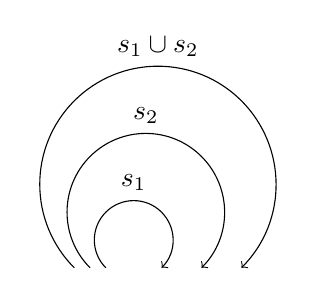
\begin{tikzpicture}
\path (0, 0) node (obj) {$\bigstar$};
\draw[->] (-0.2, 0) arc[radius=5mm, start angle=225, end angle=-45] node[pos=0.5, above]{$s_1$};
\draw[->] (-0.4, 0) arc[radius=10mm, start angle=225, end angle=-45] node[pos=0.5, above]{$s_2$};
\draw[->] (-0.6, 0) arc[radius=15mm, start angle=225, end angle=-45] node[pos=0.5, above]{$s_1 \cup s_2$};
\end{tikzpicture}
\captionsetup{labelformat=empty}
\end{figure}

接下来我们看自然数加法幺半群。任何自然数$n$,都可以用来定义一个箭头:

\[
\bigstar \arrowto{n} \bigstar
\]

箭头的组合是自然数的加法。由于加法是可结合的,所以箭头的组合是可结合的。自然数0定义了恒等箭头,这是因为0加上任何自然数等于这个自然数本身。这样我们看到自然数的加法幺半群的确构成了一个范畴。

\begin{figure}[htbp]
\centering
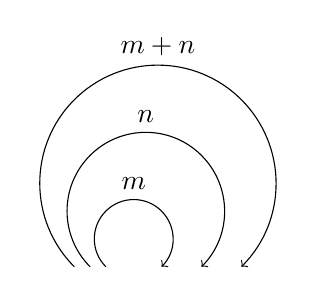
\begin{tikzpicture}
\path (0, 0) node (obj) {$\bigstar$};
\draw[->] (-0.2, 0) arc[radius=5mm, start angle=225, end angle=-45] node[pos=0.5, above]{$m$};
\draw[->] (-0.4, 0) arc[radius=10mm, start angle=225, end angle=-45] node[pos=0.5, above]{$n$};
\draw[->] (-0.6, 0) arc[radius=15mm, start angle=225, end angle=-45] node[pos=0.5, above]{$m + n$};
\end{tikzpicture}
\captionsetup{labelformat=empty}
\end{figure}


\item {第一章中我们介绍了自然数的皮亚诺公理,并且介绍了和皮亚诺算术同构的其它结构,例如链表等。这些完全可以用范畴来解释。这一结论是德国数学家戴德金发现的,尽管当时还没有范畴论。我们今天将这一范畴命名为皮亚诺范畴$\pmb{Pno}$。范畴中的对象为$(A, f, z)$,其中$A$为元素的集合,对于自然数来说这个集合是全体自然数$N$;$f: A \to A$是后继函数,对于自然数来说,就是$succ$;$z \in A$是起始元素,对于自然数来说是0。任给两个皮亚诺对象$(A, f, z)$和$(B, g, c)$,现在定义从$A$到$B$的态射
\[
A \arrowto{\phi} B
\]
它满足

\[
\phi \circ f = g \circ \phi \quad \text{且} \quad \phi(z) = c
\]

试验证$\pmb{Pno}$的确是一个范畴。}

皮亚诺范畴中的对象是$(A, f, z)$这样的三元组。箭头为保持三元组结构的映射$\phi$。箭头的组合,就是函数的组合:

\[ \begin{array}{l}
A \arrowto{\phi} B \arrowto{\psi} C \\
A \arrowto{\psi \circ \phi} C
\end{array}\]

由于函数的组合是可结合的,故箭头也是可结合的。接下来我们验证恒等箭头:

\[
A \arrowto{id_A} A
\]

它满足$id_A(z) = z$,并且$id_A \circ f = f \circ id_A$。

显然三元组$(\pmb{N}, succ, 0)$是皮亚诺范畴中的对象。并且有趣的是,对于任何皮亚诺范畴的对象$(A, f, z)$都存在唯一的箭头:

\[
(\pmb{N}, succ, 0) \arrowto{\sigma} (A, f, z)
\]

其中:

\[
\sigma(n) = f^n(z)
\]

它把任何自然数$n$映射到把$f$重复应用到$z$上$n$次。

\item {请使用叠加操作$foldr$来定义列表函子的箭头映射。}

本质上就是用$foldr$定义列表的逐一映射:

\[
fmap\ f = foldr\ f\ Nil
\]

\item {证明可能函子和列表函子的组合$\mathbf{Maybe} \circ \mathbf{List}$与$\mathbf{List} \circ \mathbf{Maybe}$仍然是函子。}

我们只证明$\mathbf{Maybe} \circ \mathbf{List}$仍然是函子。另一证明与此类似。任何对象$A$被映射为$\mathbf{Maybe} (\mathbf{List}\ A)$。对于箭头,我们先看恒等箭头的情况:

\bre
(\mathbf{Maybe} \circ \mathbf{List})\ id & = & \mathbf{Maybe} (\mathbf{List}\ id) & \text{函子的组合} \\
 & = & \mathbf{Maybe}\ id & \text{列表函子的恒等箭头} \\
 & = & id & \text{可能函子的恒等箭头} \\
\ere

然后是箭头组合:

\bre
(\mathbf{Maybe} \circ \mathbf{List})\ (f \circ g) & = & \mathbf{Maybe} (\mathbf{List}\ (f \circ g)) & \text{函子的组合} \\
 & = & \mathbf{Maybe} ((\mathbf{List}\ f) \circ (\mathbf{List}\ g)) & \text{列表函子的箭头组合性质} \\
 & = & (\mathbf{Maybe}\ (\mathbf{List}\ f)) \circ (\mathbf{Maybe}\ (\mathbf{List}\ g)) & \text{可能函子的箭头组合性质} \\
 & = & ((\mathbf{Maybe} \circ \mathbf{List})\ f) \circ ((\mathbf{Maybe} \circ \mathbf{List})\ g) & \text{函子的组合} \\
\ere

\item {证明任意函子的组合$\mathbf{G} \circ \mathbf{F}$仍然是函子。}

仿照前一题,我们分别函子的组合满足恒等箭头,和箭头组合的性质即可。首先是恒等箭头性质:

\bre
(\mathbf{G} \circ \mathbf{F})\ id & = & \mathbf{G} (\mathbf{F}\ id) & \text{函子的组合} \\
 & = & \mathbf{Maybe}\ id & \text{函子$\mathbf{F}$的恒等箭头} \\
 & = & id & \text{函子$\mathbf{G}$的恒等箭头} \\
\ere

然后是箭头组合:

\bre
(\mathbf{G} \circ \mathbf{F})\ (\phi \circ \psi) & = & \mathbf{G} (\mathbf{F}\ (\phi \circ \psi)) & \text{函子的组合} \\
 & = & \mathbf{G} ((\mathbf{F}\ \phi) \circ (\mathbf{F}\ \psi)) & \text{函子$\mathbf{F}$的箭头组合性质} \\
 & = & (\mathbf{G}\ (\mathbf{F}\ \phi)) \circ (\mathbf{G}\ (\mathbf{F}\ \psi)) & \text{函子$\mathbf{G}$的箭头组合性质} \\
 & = & ((\mathbf{G} \circ \mathbf{F})\ \phi) \circ ((\mathbf{G} \circ \mathbf{F})\ \psi) & \text{函子的组合} \\
\ere

\item {思考一个预序集范畴上的函子的例子。}

预序集范畴上的函子是一个单调映射。
% monotone function(map)

\item {回顾第二章中介绍的二叉树,请定义一个二叉树函子。}

考虑集合全函数范畴上的对象$A$,二叉树函子将其映射为:

\lstset{language=Haskell, frame=none}
\begin{lstlisting}
data Tree A = Empty | Branch (Tree A) A (Tree A)
\end{lstlisting}

对于箭头$A \arrowto{f} B$,二叉树函子将其映射为:

\bre
fmap\ f\ Empty & = & Empty \\
fmap\ f\ (Branch\ l\ x\ r) & = & Branch\ (fmap\ f\ l)\ (f\ x)\ (fmap\ f\ r) \\
\ere

或者利用第二章定义的$mapt$:

\[
fmap = mapt
\]

\item {考虑偏序集(poset)中的两个对象,它们的积是什么?余积是什么?}

第三章中,我们说到一个偏序集本身就是一个范畴,每个元素都是一个对象,任何两个对象间最多有一个箭头(如果有序关系,则存在箭头)。对于偏序集中的两个元素(对象)$a$和$b$,如果它们都有指向上下游的箭头,则

\[
\text{交运算meet}\ a \land b \quad \quad \quad \text{并运算join}\ a \lor b
\]

是这一对对象的

\[
\text{积} \quad \quad \quad \text{余积}
\]

其中交运算是两个对象的最小上界,而并运算是两个对象的最大下界。由于最小上界和最大下界并不一定存在,所以偏序集中任何两个对象的积和余积也并不一定存在。

% https://en.wikipedia.org/wiki/Join_and_meet
%In mathematics, specifically order theory, the join and meet of a subset S of a partially ordered set P are respectively the supremum (least upper bound) of S, denoted ⋁S, and infimum (greatest lower bound) of S, denoted ⋀S. In general, the join and meet of a subset of a partially ordered set need not exist. Join and meet are dual to one another with respect to order inversion.

%\item {考虑集合范畴$\pmb{Set}$,积中的两个箭头$fst, snd$是右消去(epic)的么?余积中的两个箭头$left, right$是左消去(monic)的么?}
\item {证明余积的吸收率,并验证余积函子的组合性质。}

余积的吸收率是:

\[
[p, q] \circ (f + g) = [p \circ f, q \circ g]
\]

\begin{proof}
\blre
  & [p, q] \circ (f + g)  \\
= & [p, q] \circ [left \circ f, right \circ g] & \text{$+$的定义} \\
= & [[p, q] \circ (left \circ f), [p, q] \circ (right \circ g)] & \text{余积的融合律} \\
= & [[p, q] \circ left \circ f, [p, q] \circ right \circ g] & \text{结合性} \\
= & [p \circ f, q \circ g] & \text{余积的消去律} \\
\elre
\end{proof}

余积函子的组合性质:

\[
 (f + g) \circ (f' + g') = f \circ f' + g \circ g'
\]

\begin{proof}
令$p = left \circ f$,$q = right \circ g$

\blre
  & (f + g) \circ (f' + g') \\
= & [left \circ f, right \circ g] \circ (f' + g') & \text{$+$的定义} \\
= & [p, q] \circ (f' + g') & \text{用$p, q$代换} \\
= & [p \circ f', q \circ g'] & \text{余积的吸收律} \\
= & [left \circ f \circ f', right \circ g \circ g'] & \text{把$p, q$代回} \\
= & [left \circ (f \circ f'), right \circ (g \circ g')] & \text{结合律} \\
= & f \circ f' + g \circ g' & \text{反向用$+$的定义} \\
\elre
\end{proof}

\item {证明$swap$满足自然变换的条件$(g \times f) \circ swap = swap \circ (f \times g)$}

对于$A \arrowto{f} C$和$B \arrowto{g} D$,我们要证明下面的范畴图可交换。

\begin{center}
\begin{tikzpicture}
  \matrix (m) [matrix of math nodes,
               row sep=3em, column sep=5em, minimum width=2em]{
     (A, B) & (B, A) \\
     (C, D) & (D, C) \\};
  \path[-stealth]
    (m-1-1) edge node [above] {$swap_{A, B}$} (m-1-2)
    (m-2-1) edge node [below] {$swap_{C, D}$} (m-2-2)
    (m-1-1) edge node [left] {$f \times g$} (m-2-1)
    (m-1-2) edge node [right] {$g \times f = swap\ f \times g$} (m-2-2);
\end{tikzpicture}
\end{center}

\begin{proof}
\blre
  & ((g \times f) \circ swap)\ (A, B) \\
= & (g \times f)\ (swap\ (A, B)) & \text{组合的定义} \\
= & (g \times f) \circ (B, A) & \text{$swap$的定义} \\
= & (g\ B, f\ A) & \text{箭头的积} \\
= & (D, C) & \text{箭头$g, f$的定义} \\
= & swap\ (C, D) & \text{反向用$swap$的定义} \\
= & swap\ (f\ A, g\ B) & \text{反向用$f, g$的定义} \\
= & swap\ ((f \times g)\ (A, B)) & \text{箭头的积} \\
= & (swap \circ (f \times g))\ (A, B) & \text{反向用组合的定义} \\
\elre
\end{proof}

\item {证明多态函数$length$是一个自然变换,其定义如下:
\[
\begin{array}{l}
length : [A] \to Int \\
length\ [] = 0 \\
length\ (x:xs) = 1 + length\ xs
\end{array}
\]
}

对于任何对象$A$,它的索引箭头$length$为:

\[
[A] \arrowto{length_A} \mathbf{K}_{Int}\ A
\]

其中$\mathbf{K}_{Int}$是常函子,它将任何对象映射到$Int$,所有箭头映射为恒等箭头$id_{int}$。对于箭头$A \arrowto{f} B$,我们要证明下面的范畴图可交换。

\begin{center}
\begin{tikzpicture}
  \matrix (m) [matrix of math nodes,
               row sep=3em, column sep=5em, minimum width=2em]{
     A & \lbrack A \rbrack & \mathbf{K}_{Int}\ A \\
     B & \lbrack B \rbrack & \mathbf{K}_{Int}\ B \\};
  \path[-stealth]
    (m-1-1) edge node [left] {$f$} (m-2-1)
    % square
    (m-1-2) edge node [above] {$length_A$} (m-1-3)
    (m-2-2) edge node [below] {$length_B$} (m-2-3)
    (m-1-2) edge node [left] {$\mathbf{List}(f)$} (m-2-2)
    (m-1-3) edge node [right] {$\mathbf{K}_{Int}(f)$} (m-2-3);
\end{tikzpicture}
\end{center}

利用常函子的定义,这个范畴图等价于:

\begin{center}
\begin{tikzpicture}
  \matrix (m) [matrix of math nodes,
               row sep=3em, column sep=5em, minimum width=2em]{
     A & \lbrack A \rbrack & Int \\
     B & \lbrack B \rbrack & Int \\};
  \path[-stealth]
    (m-1-1) edge node [left] {$f$} (m-2-1)
    % square
    (m-1-2) edge node [above] {$length_A$} (m-1-3)
    (m-2-2) edge node [below] {$length_B$} (m-2-3)
    (m-1-2) edge node [left] {$\mathbf{List}(f)$} (m-2-2)
    (m-1-3) edge node [right] {$id$} (m-2-3);
\end{tikzpicture}
\end{center}

也就是要证明:

\[
id \circ length_{A} = length_{B} \circ \mathbf{List}(f)
\]

即:$length_{A} = length_{B} \circ \mathbf{List}(f)$


\begin{proof}
我们用数学归纳法证明。首先是空列表:

\blre
  & length_B \circ \mathbf{List}(f) [] \\
= & length_B [] & \text{列表函子的定义} \\
= & 0 & \text{$length$的定义} \\
= & length_A\ [] & \text{反向用$length$的定义}
\elre

然后是归纳假设,设$length_B \circ \mathbf{List}(f)\ as = length_A\ as$成立,我们有:

\blre
  & length_B \circ \mathbf{List}(f) (a:as) \\
= & length_B\ (f(a) : \mathbf{List}(f)\ as) & \text{列表函子的定义} \\
= & 1 + length_B\ (\mathbf{List}(f)\ as) & \text{$length$的定义} \\
= & 1 + length_B\ \circ \mathbf{List}(f)\ as & \text{箭头组合} \\
= & 1 + length_A\ as & \text{归纳假设} \\
= & length_A\ (a:as) & \text{反向用$length$的定义}
\elre
\end{proof}

\item {自然变换也可以进行组合,考虑两个自然变换$\mathbf{F} \arrowto{\phi} \mathbf{G}$和$\mathbf{G} \arrowto{\psi} \mathbf{H}$,对于任意箭头$A \arrowto{f} B$,试画出自然变换组合$\phi \circ \psi$的范畴图,并列出可交换性的条件。}

\begin{center}
\begin{tikzpicture}
  \matrix (m) [matrix of math nodes,
               row sep=3em, column sep=5em, minimum width=2em]{
     \mathbf{F}A & \mathbf{G}A & \mathbf{H}A \\
     \mathbf{F}B & \mathbf{G}B & \mathbf{H}B \\};
  \path[-stealth]
    (m-1-1) edge node [left] {$\mathbf{F}(f)$} (m-2-1)
    (m-1-1) edge node [above] {$\phi_A$} (m-1-2)
    (m-2-1) edge node [below] {$\phi_B$} (m-2-2)
    (m-1-2) edge node [above] {$\psi_A$} (m-1-3)
    (m-2-2) edge node [below] {$\psi_B$} (m-2-3)
    (m-1-2) edge node [left] {$\mathbf{G}(f)$} (m-2-2)
    (m-1-3) edge node [right] {$\mathbf{H}(f)$} (m-2-3);
\end{tikzpicture}
\end{center}

可交换的条件为:

\[
\mathbf{H}(f) \circ (\psi_A \circ \phi_A) = (\psi_B \circ \phi_B) \circ \mathbf{F} (f)
\]

\item{在本节的例子中,我们说在一个偏序集中,如果存在最小值(或最大值),则最小值(或最大值)就是起始对象(或终止对象)。考虑全体偏序集构成的范畴$\pmb{Poset}$,如果存在起始对象,它是什么?如果存在终止对象,它是什么?}

对于$\pmb{Poset}$范畴,对象是偏序集,箭头是单调映射。对于两个偏序集$P, Q$,箭头$P \arrowto{h} Q$使得偏序集$P$中任何两个有序元素$a \leq b$,有$h(a) \leq h(b)$。

这一范畴中的起始对象是空偏序集$0 = \varnothing$。它到任何其它偏序集有唯一的箭头:

\[
\varnothing \longrightarrow P
\]

终止对象是之后一个元素的偏序集$1 = \{\bigstar\}$,偏序关系为$R = \{(\bigstar, \bigstar)\}$,即$\bigstar \leq \bigstar$。任何偏序集$P$到1有唯一的箭头:

\bre
P & \longrightarrow & \{\bigstar\} \\
p & \mapsto & \bigstar
\ere

\item{皮亚诺范畴$\pmb{Pno}$(参见本章第一节的习题2)中,什么样的对象$(A, f, z)$是起始对象?终止对象是什么?}

起始对象是$(\pmb{N}, succ, 0)$,它到任何其它对象唯一箭头是:

\[
(\pmb{N}, succ, 0) \arrowto{\sigma} (A, f, z): \sigma(n) = f^n(z)
\]

终止对象是只有一个元素的对象$1 = (\{\bigstar\}, \bigstar, id)$。任何皮亚诺范畴的对象$(A, f, z)$到终止对象的唯一箭头是:

\[
(A, f, z) \arrowto{\sigma} 1 : \sigma(a) = \bigstar
\]

\item{验证$\pmb{Exp}$的确是一个范畴,指出$id$箭头和箭头的组合。}

我们先看$id$箭头的定义$h \arrowto{id} h$,它使得下面的范畴图可交换:

\begin{center}
\begin{tikzpicture}
  \matrix (m) [matrix of math nodes,
               row sep=3em, column sep=5em, minimum width=2em]{
     A & A \times B & \\
     A & A \times B & C \\};
  \path[-stealth]
    (m-1-1) edge node [left] {$id_A$} (m-2-1)
    (m-1-2) edge node [left] {$id_A \times id_B$} (m-2-2)
    (m-1-2) edge node [above] {$h$} (m-2-3)
    (m-2-2) edge node [below] {$h$} (m-2-3);
\end{tikzpicture}
\end{center}

然后是箭头组合:

$h \arrowto{i} k$和$k \arrowto{j} m$的组合是$j \circ i$使得下面的范畴图交换:

\begin{center}
\begin{tikzpicture}
  \matrix (m) [matrix of math nodes,
               row sep=3em, column sep=5em, minimum width=2em]{
     A & A \times B & \\
     D & D \times B & C \\
     E & E \times B & \\};
  \path[-stealth]
    (m-1-1) edge node [left] {$f$} (m-2-1)
    (m-2-1) edge node [left] {$g$} (m-3-1)
    (m-1-2) edge node [left] {$f \times id_B$} (m-2-2)
    (m-2-2) edge node [left] {$g \times id_B$} (m-3-2)
    (m-1-2) edge node [above] {$h$} (m-2-3)
    (m-2-2) edge node [above] {$k$} (m-2-3)
    (m-3-2) edge node [below] {$m$} (m-2-3);
\end{tikzpicture}
\end{center}

因此对于箭头$h \arrowto{j} k$有:$id_k \circ j = j = j \circ id_h$。并且对于三个箭头有结合律。

\item{反射律$curry\ apply = id$中,$id$的下标是什么?请用另一种方法证明它。}

$id$的下标是二元箭头的类型$A \times B \to C$。

\begin{proof}
\blre
  & curry \circ apply\ f\ a\ b \\
= & curry\ (apply\ f)\ a\ b & \text{组合的定义} \\
= & (apply\ f)\ (a, b) & \text{$curry$的定义}\\
= & f(a, b) & \text{$apply$的定义} \\
= & id_{A \times B \to C}\ f(a, b)
\elre
\end{proof}

\item{我们称下面的等式
\[
(curry\ f) \circ g = curry(f \circ (g \times id))
\]
为克里化的融合律。请画出它的范畴图并证明它。}

\begin{center}
\begin{tikzpicture}
  \matrix (m) [matrix of math nodes,
               row sep=3em, column sep=5em, minimum width=2em]{
     D & D \times B & \\
     A & A \times B & \\
     C^B & C^B \times B & C \\};
  \path[-stealth]
    (m-1-1) edge node [left] {$g$} (m-2-1)
    (m-2-1) edge node [left] {$curry\ f$} (m-3-1)
    (m-1-2) edge node [left] {$g \times id$} (m-2-2)
    (m-1-2) edge [bend right] node {} (m-3-2)
    (m-1-2) edge node [above] {$f \circ (g \times id)$} (m-3-3)
    (m-2-2) edge node [above] {$f$} (m-3-3)
    (m-3-2) edge node [below] {$apply$} (m-3-3);
\end{tikzpicture}
\end{center}

观察图中$D \times B$,$A \times B$,和$C$这个三角形。我们知道$D \times B \to A$这个组合箭头为$f \circ (g \times id)$。

根据幂对象和转换箭头的定义有:

\[
apply \circ (curry f) \circ g = f \circ (g \times id)
\]

由$curry$和$apply$的泛性性质有:

\[
(curry f) \circ g = curry (f \circ (g \times id)
\]

\item{画出群的可逆性公理的范畴图。}

可逆性公里表示为:$m \circ (id, i) = m \circ (i, id) = e$

\begin{center}
\begin{tikzpicture}
  \matrix (m) [matrix of math nodes,
               row sep=3em, column sep=5em, minimum width=2em]{
     G & G \times G & G \\
     1 & G & 1 \\};
  \path[-stealth]
    (m-1-1) edge node [above] {$(id, i)$} (m-1-2)
    (m-1-3) edge node [above] {$(i, id)$} (m-1-2)
    (m-1-1) edge node [left] {} (m-2-1)
    (m-1-2) edge node [left] {$m$} (m-2-2)
    (m-1-3) edge node [left] {} (m-2-3)
    (m-2-1) edge node [above] {$e$} (m-2-2)
    (m-2-3) edge node [above] {$e$} (m-2-2);
\end{tikzpicture}
\end{center}

\item{$p$是一个素数,使用群的F-代数,为整数模$p$乘法群(可以参考上一章)定义一个$\alpha$箭头。}

根据群的$\alpha$箭头定义:

\[
\mathbf{F} A \arrowto{\alpha = e + m +i} A
\]
定义整数模$p$乘法群如下:

\bre
e\ () & = & 1 & \text{单位元是1} \\
m(a, b) & = & ab \bmod p & \text{二元运算是模$p$乘法} \\
i(a) & = & a^{p-2} \bmod p & \text{根据费马小定理$a^{p-1} \equiv 1 \mod p$} \\
\ere

\item{参考上一章环的定义,定义环的F-代数。}

环上的代数结构由三部分组成:
\begin{enumerate}[i]
\item 携带对象$R$,用于携带环上代数结构的集合。
\item 多项式函子$\mathbf{F}A = 1 + 1 + A \times A + A \times A + A$。
\item 箭头$\mathbf{F}A \arrowto{\alpha = z + e + p + m + n} A$,它们分别是加法单位元$z$,乘法单位元$e$,加法$p$,乘法$m$,和求反$n$。
\end{enumerate}
这样就定义了一个环上的$F$-代数$(R, \alpha)$。例如当携带对象是整数时,算术运算下的环定义为:

\[\begin{array}{l}
z\ () = 0 \\
e\ () = 1 \\
p(a, b) = a + b \\
m(a, b) = ab \\
n(a) = -a \\
\end{array}\]

\item{F-代数范畴上的$id$箭头是什么?箭头组合是什么?}

从$F$-代数$(A, \alpha)$到其自身的同态映射是$id$箭头。箭头组合是$F$-态射的组合。携带对象间的箭头:$A \arrowto{f} B \arrowto{g} C$使得下面的范畴图可交换:

\begin{center}
\begin{tikzpicture}
  \matrix (m) [matrix of math nodes,
               row sep=3em, column sep=5em, minimum width=2em]{
     \mathbf{F} A & \mathbf{F} B & \mathbf{F} C \\
     A & B & C \\};
  \path[-stealth]
    (m-1-1) edge node [left] {$\alpha$} (m-2-1)
    (m-1-2) edge node [left] {$\beta$} (m-2-2)
    (m-1-3) edge node [left] {$\gamma$} (m-2-3)
    (m-1-1) edge node [above] {$\mathbf{F}(f)$} (m-1-2)
    (m-1-2) edge node [above] {$\mathbf{F}(g)$} (m-1-3)
    (m-2-1) edge node [below] {$f$} (m-2-2)
    (m-2-2) edge node [below] {$g$} (m-2-3);
\end{tikzpicture}
\end{center}

\[
  g \circ f \circ \alpha = \gamma \circ \mathbf{F}(g) \circ \mathbf{F}(f) = \gamma \circ \mathbf{F}(g \circ f)
\]

\item{可否把类自然数函子写成如下递归的形式?谈谈你的看法。
\begin{lstlisting}
data NatF A = ZeroF | SuccF (NatF A)
\end{lstlisting}
}

不可以。考虑携带对象$A$,上述函子$\mathbf{NatF}$是迭代的,它并不将$A$映射为确定的某个对象。事实上,我们希望把它映射为皮亚诺范畴上的对象$(A, z, f)$。

\item{我们可以为$\mathbf{NatF} Int \to Int$定义一个$\alpha$箭头,名叫$eval$:
\[
\begin{array}{l}
eval : \mathbf{NatF} Int \to Int \\
eval\ ZeroF = 0 \\
eval\ (SuccF\ n) = n + 1 \\
\end{array}
\]
如果迭代地将$A' = \mathbf{NatF} A$代入$\mathbf{NatF}$函子$n$次。我们把这样得到的函子记为$\mathbf{NatF}^n A$。试思考能否定义下面的$\alpha$箭头:
\[
\begin{array}{l}
eval : \mathbf{NatF}^n Int \to Int \\
\end{array}
\]
}

\bre
eval & : &\mathbf{NatF}^n Int \to Int \\
eval\ ZeroF & = & 0 & \text{$ZeroF$是$\mathbf{NatF}^n Int$的对象}\\
eval\ (SuccF\ ZeroF) & = & 1 & \text{$ZeroF$是$\mathbf{NatF}^{n-1} Int$的对象}\\
eval\ (SuccF\ (SuccF\ ZeroF)) & = & 2 & \text{$ZeroF$是$\mathbf{NatF}^{n-2} Int$的对象}\\
... \\
eval\ (SuccF^{n-1}\ ZeroF) & = & n - 1 & \text{$ZeroF$是$\mathbf{NatF} Int$的对象}\\
eval\ (SuccF^n\ m) & = & m + n \\
\ere

\item{对二叉树函子$\mathbf{TreeF}\ A\ B$,固定$A$,利用不动点验证$(\mathbf{Tree}\ A, [nil, branch])$是初始代数。}

令$B' = \mathbf{TreeF}\ A\ B$,然后不断递归地应用到自己,把此结果称为$\mathbf{Fix}\ (\mathbf{TreeF}\ A)$。

\bre
\mathbf{Fix}\ (\mathbf{TreeF}\ A) & = & \mathbf{TreeF}\ A\ (\mathbf{Fix}\ (\mathbf{TreeF}\ A)) & \text{不动点的定义} \\
 & = & \mathbf{TreeF}\ A\ (\mathbf{TreeF}\ A (...)) & \text{递归展开} \\
 & = & NilF | BrF\ A\ (\mathbf{TreeF}\ A\ (...))\ (\mathbf{TreeF}\ A\ (...)) & \text{二叉树函子的定义} \\
 & = & NilF | BrF\ A\ (\mathbf{Fix}\ (\mathbf{TreeF}\ A))\ (\mathbf{Fix}\ (\mathbf{TreeF}\ A)) & \text{反向用不动点} \\
\ere

比较$Tree A$的定义:

\begin{lstlisting}
data Tree A = Nil | Br A (Tree A) (Tree A)
\end{lstlisting}

故而:$\mathbf{Tree}\ A = \mathbf{Fix}\ (\mathbf{TreeF}\ A)$。初始代数为$(\mathbf{Tree}\ A, [nil, branch])$。

\end{enumerate}

\section{融合}

\begin{enumerate}
\item {验证从左侧叠加也可以表示为$foldr$:
\[
foldl\ f\ z\ xs = foldr\ (b\ g\ a \mapsto g\ (f\ a\ b))\ id\ xs\ z
\]}

为了方便理解,我们将其改写为:

\[\begin{array}{l}
foldl\ f\ z\ xs = foldr\ step\ id\ xs\ z \\
\text{其中:} step\ x\ g\ a = g\ (f\ a\ x)
\end{array}\]

\blre
  & foldl\ f\ z\ [x_1, x_2, ..., x_n] \\
= & (foldr\ step\ id\ [x_1, x_2, ..., x_n])\ z \\
= & (step\ x_1 (step\ x_2 ( ... (step\ x_n\ id))) ...)\ z \\
= & (step\ x_1 (step\ x_2 ( ... (a_n \mapsto id\ (f\ a_n\ x_n)))) ...)\ z \\
= & (step\ x_1 (step\ x_2 ( ...(a_{n-1} \mapsto (a_n \mapsto id\ (f\ a_n\ x_n))\ (f\ a_{n-1}\ x_{n-1}))))...)\ z \\
= & (a_1 \mapsto (a_2 \mapsto ( ... (a_n \mapsto id\ (f\ a_n\ x_n))\ (f\ a_{n-1}\ x_{n-1})) ... (f\ a_2\ x_2)) (f\ a_1\ x_1))\ z \\
= & (a_1 \mapsto (a_2 \mapsto ( ... (a_n \mapsto f\ a_n\ x_n)\ (f\ a_{n-1}\ x_{n-1})) ... )\ (f\ a_1\ x_1))\ z \\
= & (a_1 \mapsto (a_2 \mapsto (... (a_{n-1} \mapsto f\ (f\ a_{n-1}\ x_{n-1})\ x_n)\ ...))\ (f\ a_1\ x_1))\ z \\
= & (a_1 \mapsto f\ (f\ (...(f\ a_1\ x_1)\ x_2)\ ...)\ x_n)\ z \\
= & f\ (f\ (...(f\ z\ x_1)\ x_2)\ ...)\ x_n
\elre

如果把$f$改写成$\oplus$,并写成中缀形式,就能看出$foldl$和$foldr$的区别:

\[
foldl\ \oplus\ f\ z = ((...(z \oplus x_1)\ \oplus x_2)...)\ \oplus x_n
\]

\item {证明以下列表的构建——叠加形式:
\[
\begin{array}{l}
concat\ xss = build\ (f\ z \mapsto foldr\ (xs\ x \mapsto foldr\ f\ x\ xs)\ xss) \\
map\ f\ xs = build\ (\oplus\ z \mapsto foldr\ (y\ ys \mapsto (f\ y) \oplus ys)\ z\ xs) \\
filter\ f\ xs = build\ (\oplus\ z \mapsto foldr\ (x\ xs' \mapsto
  \begin{cases}
     f(x): & x \oplus xs' \\
    \text{否则}: & xs' \\
  \end{cases})\ z\ xs) \\
repeat\ x = build\ (\oplus\ z \mapsto let\ r = x \oplus r\ in\ r) \\
\end{array}
\]
}

首先是多个列表的连接$concat$
\begin{proof}
\blre
  & build\ (f\ z \mapsto foldr\ (xs\ x \mapsto foldr\ f\ x\ xs)\ z\ xss) \\
= & (f\ z \mapsto foldr\ (xs\ x \mapsto foldr\ f\ x\ xs)\ z\ xss)\ (:)\ [] & \text{$build$的定义} \\
= & foldr\ (xs\ x \mapsto foldr\ (:)\ x\ xs)\ []\ xss & \text{$\beta$-规约} \\
= & foldr\ \doubleplus []\ xss & \text{两个列表连接的定义} \\
= & concat\ xss & \text{多列表连接的定义} \\
\elre
\end{proof}

接着是逐一映射$map$
\begin{proof}
\blre
  & build\ (\oplus\ z \mapsto foldr\ (y\ ys \mapsto (f\ y) \oplus ys)\ z\ xs) \\
= & (\oplus\ z \mapsto foldr\ (y\ ys \mapsto (f\ y) \oplus ys)\ z\ xs)\ (:)\ [] & \text{$build$的定义} \\
= & foldr\ (y\ ys \mapsto f(y) : ys)\ []\ xs & \text{$\beta$-规约} \\
= & foldr\ (x\ ys \mapsto f(x) : ys)\ []\ xs & \text{$\alpha$变换,改名字} \\
= & map\ f\ xs & \text{逐一映射的定义} \\
\elre
\end{proof}

接着是过滤操作$filter$

\begin{proof}
\blre
  & build\ (\oplus\ z \mapsto foldr\ (x\ xs' \mapsto
  \begin{cases}
     f(x): & x \oplus xs' \\
    \text{否则}: & xs' \\
  \end{cases})\ z\ xs) \\
= & (\oplus\ z \mapsto foldr\ (x\ xs' \mapsto
  \begin{cases}
     f(x): & x \oplus xs' \\
    \text{否则}: & xs' \\
  \end{cases})\ z\ xs)\ (:)\ [] & \text{$build$的定义} \\
= & foldr\ (x\ xs' \mapsto
  \begin{cases}
     f(x): & x : xs' \\
    \text{否则}: & xs' \\
  \end{cases})\ []\ xs & \text{$\beta$-规约} \\
= & filter\ f\ xs & \text{过滤操作的定义} \\
\elre
\end{proof}

最后是重复操作$repeat$

\begin{proof}
\blre
  & build\ (\oplus\ z \mapsto let\ r = x \oplus r\ in\ r) \\
= & (\oplus\ z \mapsto let\ r = x \oplus r\ in\ r)\ (:)\ [] & \text{$build$的定义} \\
= & (let\ r = x : r\ in\ r) & \text{$\beta$-规约} \\
= & repeat\ x & \text{重复操作的定义} \\
\elre
\end{proof}

\item{化简快速排序算法:
\[
\begin{cases}
qsort\ [] = [] \\
qsort\ (x:xs) = qsort\ [a | a \in xs, a \leq x] \doubleplus [x] \doubleplus qsort\ [a | a \in xs, x < a] \\
\end{cases}\]
}

可以把ZF表达式变换成$filter$。显然这里处理了两遍列表,它们可以合成一次:

\[
\begin{cases}
qsort\ [] & = [] \\
qsort\ (x:xs) & = qsort\ as \doubleplus [x] \doubleplus qsort\ bs \\
\end{cases}
\]

其中:
\[\begin{array}{l}
(as, bs) = foldr\ h\ ([], [])\ xs \\
h\ y\ (as', bs') = \begin{cases}
               y \leq x : & (y:as', bs') \\
               \text{否则}: & (as', y:bs') \\
\end{cases} \\
\end{array}\]

接下来我们可以把两个列表的连接操作化简:

\blre
  & qsort\ as \doubleplus [x] \doubleplus qsort\ bs \\
= & qsort\ as \doubleplus (x : qsort\ bs) \\
= & foldr (:)\ (x : qsort\ bs) (qsort\ as)
\elre

\item{利用范畴论验证融合律的类型限制。提示:考虑向下态射的类型。}

观察范畴图:

\begin{center}
\begin{tikzpicture}
  \matrix (m) [matrix of math nodes,
               row sep=3em, column sep=5em, minimum width=2em]{
     \mathbf{ListF} A\ \lbrack A \rbrack & \lbrack A \rbrack \\
     \mathbf{ListF} A\ B\ & B \\};
  \path[-stealth]
    (m-1-1) edge node [left] {$\mathbf{ListF} A(h)$} (m-2-1)
    (m-1-2) edge node [right] {$h = \lbb \alpha \rbb$} (m-2-2)
    (m-1-1) edge node [above] {$(:) + []$} (m-1-2)
    (m-2-1) edge node [below] {$\alpha = f + z$} (m-2-2);
\end{tikzpicture}
\end{center}

向下态射$\lbb \alpha \rbb$被抽象成从$\alpha$构造某种代数结构$g\ \alpha$。$g$接受一个$F$-代数的$\alpha$箭头,产生结果$B$。$\alpha$箭头是$f : A \to B \to B$和$z : 1 \to B$的余积。故其类型为:

\[
g : \forall A. (\forall B. (A \to B \to B) \to B \to B)
\]

构造的定义是$build(g) = g\ (:)\ []$,它把$g$应用到初始代数的$\alpha$箭头上从而构造出初始代数中的对象,也就是列表$[A]$。因而:

\[
build : \forall A. (\forall B. (A \to B \to B) \to B \to B) \to \mathbf{List}\ A
\]

\item{利用融合律化简算式求值的定义$eval = sum \circ map\ (product \circ (map\ dec))$。}

\blre
  & eval es \\
= & sum (map\ (product \circ (map\ dec))\ es) & \text{函数组合} \\
  & \{ \text{$sum$展开为叠加形式,$map$展开为构建形式} \} \\
= & \pmb{foldr}\ (+)\ 0\ (\pmb{build}\ (\oplus\ z\ \mapsto foldr\ (t\ ts \mapsto (f\ t) \oplus ts)\ z\ es)) & \text{令$f = product \circ (map\ dec)$} \\
= & (\oplus\ z \mapsto foldr\ (t\ ts \mapsto (f\ t) \oplus ts)\ z\ es)\ (+)\ 0 & \text{融合律} \\
= & foldr\ (t\ ts \mapsto (f t) + ts)\ 0\ es & \text{$\beta$规约} \\
\elre

写成无参数形式就是:

\[
eval = foldr\ (t\ ts \mapsto (f\ t) + ts)\ 0
\]

接下来我们再化简$product \circ (map\ dec)$部分

\blre
  & (product \circ (map\ dec))\ t \\
= & product\ (map\ dec\ t) & \text{函数组合} \\
  & \{ \text{$product$展开为叠加形式,$map$展开为构建形式} \} \\
= & \pmb{foldr}\ (\times)\ 1\ (\pmb{build}\ (\oplus\ z \mapsto foldr\ (d\ ds \mapsto (dec\ d) \oplus ds)\ z\ t)) \\
= & (\oplus\ z \mapsto foldr (d\ ds \mapsto (dec\ d) \oplus ds)\ z\ t)\ (\times)\ 1 & \text{融合律} \\
= & foldr\ (d\ ds \mapsto (dec\ d) \times ds)\ 1\ t & \text{$\beta$规约} \\
= & foldr\ ((\times) \circ fork\ (dec, id))\ 1\ t & \text{定义$fork(f, g)\ x = (f\ x, g\ x)$} \\
\elre

接着把这个结果代入之前的$f$,得到最终化简的结果:

\[
eval = foldr\ (t\ ts \mapsto (foldr\ ((\times) \circ fork\ (dec, id))\ 1\ t) + ts)\ 0
\]

\item{如何从左侧扩展出所有的算式?}

从左向右扩展时,针对每个数字$d$,有三种选择:

\begin{enumerate}
\item 什么都不插入意味着将数字$d$直接添加到$e_i$的最后一个子算式中的最后一个因子的后面。这样由$f_n ++ [d]$组成一个新的因子。例如$e_i$是算式$1 + 2$,数字$d$是3,将3写在$1 + 2$的后面而什么符号都不插入,这样就得到新算式$1 + 23$;
\item 插入乘号意味着用数字$d$构成一个因子$[d]$,然后将它添加到$e_i$中最后一个子算式的后面。这样由$t_m ++ [[d]]$组成一个新的子算式。具体到$1 + 2$这个例子,我们把3写在它的后面,然后在2和3之间插入一个乘号,这样就得到新算式$1 + 2 \times 3$;
\item 插入加号意味着用数字$d$构成一个子算式$[[d]]$,然后将将它添加到$e_i$的最后面,组成新的算式$e_i ++ [[[d]]]$。具体到$1 + 2$这个例子,我们把3写在它的后面,然后在2和3之间插入一个加号,这样就得到新算式$1 + 2 + 3$。
\end{enumerate}

为了将一个元素加到序列的末尾,我们可以定义一个函数:

\[
append\ x = foldr\ (:)\ [x]
\]

然后我们定义一个函数$onLast(f)$,它把$f$应用到一个序列的最后一个元素上:

\[\begin{array}{l}
onLast\ f = foldr\ h\ [] \\
\text{其中}: \begin{cases}
  h\ x\ [] & = [(f\ x)] \\
  h\ x\ xs & = x : xs \\
\end{cases} \\
\end{array}\]

然后,我们就可以实现这3种情况的扩展:

\lstset{frame = none}
\begin{lstlisting}
add d exp = [((append d) `onLast`) `onLast` exp,
             (append [d]) `onLast` exp,
             (append [[d]]) exp]
\end{lstlisting}

\item{下面定义可以将算式翻译为字符串:
\[
str = (join\ \text{``+''}) \circ (map\ ((join\ \text{``} \times \text{''}) \circ (map\ (show \circ dec))))
\]
其中$show$可以将数字转换为字符串。函数 $join(c, s)$ 将一组字符串$s$用$c$连接起来,例如 $join($``\#''$, [$``abc'', ``def''$]) = $``abc\#def'' 。利用融合律化简$str$的定义。
}

第五章中,我们给出了$join(ws)$的结果,它实际上是用空格分割一组字符串。将空格作为参数,就得到了$join(c, s)$的定义:

\[
join\ c = foldr\ (w\ b \mapsto foldr\ (:)\ (c:b)\ w)\ []
\]

观察$str$的定义,它实际上是两重的$(join\ c) \circ (map\ f)$的形式,即:

\[\begin{array}{l}
str = (join\ c) \circ (map\ f) \\
\text{其中}: f = (join\ d) \circ (map\ g) \\
\end{array}\]

这里$c = `+', d = ` \times '$,而$g = show \circ dec$。为此我们只要找出$(join\ c) \circ (map\ f)$的简化形式就可以了。

\blre
  & (join\ c) \circ (map\ f)\ es \\
  & \{ \text{$join$展开为叠加,$map$展开为构建形式} \} \\
= & \pmb{foldr}\ (w\ b \mapsto foldr\ (:) (c:b)\ w)\ [] (\pmb{build}\ (\oplus\ z \mapsto foldr\ (y\ ys \mapsto (f\ y) \oplus ys)\ z\ es)) \\
  & \{ \text{融合律} \} \\
= & (\oplus\ z \mapsto foldr\ (y\ ys \mapsto (f\ y) \oplus ys)\ z\ es))\ (w\ b \mapsto foldr\ (:)\ (c:b)\ w)\ [] \\
  & \{ \text{$\beta$规约} \} \\
= & foldr\ (y\ ys \mapsto foldr\ (:)\ (c:ys)\ (f\ y))\ []\ es \\
\elre

将之前的加号、乘号,以及$show \circ dec$代入,我们得到结果:

\blre
str & = & foldr\ (x\ xs \mapsto foldr\ (:)\ (`+':xs) ( \\
    &   & \quad foldr (y\ ys \mapsto foldr\ (:)\ (`\times':ys)\ (show \circ dec\ y))\ [])\ [] \\
\elre

\end{enumerate}

\section{无穷}

\begin{enumerate}

\item{第一章中,我们用叠加操作实现了斐波那契数列,如何用$iterate$定义斐波那契数列潜无穷?}

\[
F = (fst \circ unzip)\ (iterate\ ((m, n) \mapsto (n, m + n))\ (1, 1))
\]

例如$take\ 100\ F$

\item{用叠加操作定义$iterate$。}

我们考虑潜无穷流$iterate\ f\ x$,如果将$f$再次应用到每个元素上,并且在最前面添加一个$x$,得到的仍然是这个无穷流。基于这点我们可以定义:

\[
iterate\ f\ x = x : foldr (y\ ys \mapsto (f\ y):ys)\ []\ (iterate\ f\ x)
\]

例如:

\begin{lstlisting}
take 10 $ iter (+1) 0
[0,1,2,3,4,5,6,7,8,9]
\end{lstlisting} %$

\item{利用第四章中介绍的不动点定义,证明$Stream$是$StreamF$的不动点。}

令$A' = \mathbf{StreamF}\ E\ A$,然后不断递归地应用到自己,把此结果称为$\mathbf{Fix}\ (\mathbf{StreamF}\ E)$

\bre
\mathbf{Fix}\ (\mathbf{StreamF}\ E) & = &
    \mathbf{StreamF}\ E\ (\mathbf{Fix}\ (\mathbf{StreamF}\ E)) & \text{不动点的定义} \\
 & = & \mathbf{StreamF}\ E\ (\mathbf{StreamF}\ E\ (...)) & \text{递归展开} \\
 & = & \mathbf{Stream}\ E\ (\mathbf{Stream}\ E) & \text{替换名称} \\
 & = & \mathbf{Stream}\ E & \text{反向用$Stream$的定义} \\
\ere

故$Stream$是$StreamF$的不动点。

\item{试定义反折叠$unfold$}

在实现时,通常使用$Maybe$来定义出一个结束条件:
\begin{lstlisting}
unfold :: (b -> Maybe (a, b)) -> (b -> [a])
unfold f b = case f b of
                Just (a, b') -> a : unfold f b'
                Nothing -> []
\end{lstlisting}

\item 数论中的算术基本定理说:任何一个大于1的整数都可以唯一地表示成若干素数的乘积。有一道编程趣题,要求判断一段文字$T$中,是否包含一个字符串$W$的某种排列。试利用算术基本定理,和素数流解决这道题目。

我们的思路是,将每一个不同字符对应到一个素数上去,a对应2,b对应3,c对应5……。这样任意给定一个字符串$W$,不管它是否包含重复的字符,我们都可以把它表示为素数的乘积:

\[
F = \prod p_c , c \in W
\]

我们称其为字符串$W$的数论指纹$F$。如果$W$是空串,我们规定它的指纹等于1。根据整数乘法的交换律,我们知道无论$W$怎样排列,其数论指纹都不变,并且根据算术基本定理,这个数论指纹是唯一的。现在我们就得到了一个特别简洁的解法:我们首先计算出$W$的数论指纹$F$,然后用一个长度为$|W|$的窗口沿着$T$从左向右滑动。一开始我们需要计算$T$在这个窗口内的数论指纹,并和$F$比较,如果相等就说明$T$包含$W$的某种排列。如果不等我们将这个窗口向右滑动一个字符。此时我们可以非常容易地计算新窗口内的数论指纹:只要把滑出的字符对应的素数除掉,再把滑入的字符对应的素数乘上就可以了。任何时候如果新窗口内的数论指纹等于$F$,就说明找到了一个排列。当然为了获得每个不同字符对应的素数,我们还要利用埃拉托斯特尼筛法产生一串素数。下面是一段示例算法:

\begin{algorithmic}
\Function{contains?}{$W, T$}
  \State $P \gets ana \ era \ [2, 3, ...]$ \Comment{素数序列}
  \If{$W = \phi$}
    \State \Return True
  \EndIf
  \If{$|T| < |W|$}
    \State \Return False
  \EndIf
  \State $\displaystyle m \gets \prod P_c, c \in W$
  \State $\displaystyle m' \gets \prod P_c, c \in T[1...|W|]$
  \For{$i \gets |W| + 1$ to $|T|$}
    \If{$m = m'$}
      \State \Return True
    \EndIf
    \State $m' \gets m' \times P_{T_i} / P_{T_{i - |W|}} $
  \EndFor
  \State \Return $m = m'$
\EndFunction
\end{algorithmic}

\item{我们建立了房间和任意旅游团的客人间的一一映射。第$i$号旅游团的第$j$号客人应该入住几号房间?第$k$个房间里住了哪号旅游团的哪位客人?}

按照本章约定,从0开始计数。用数偶$(i, j)$表示第$i$号旅游图的第$j$号客人。我们列出前面的几个客人和房间的对应关系

\btab{c|c|c|c|c|c|c|c|c|c|c|c}
$(i, j)$ & (0, 0) & (0, 1) & (1, 0) & (2, 0) & (1, 1) & (0, 2) & (0, 3) & (1, 2) & (2, 1) & (3, 0) & ... \\
\hline
$k$ & 0 & 1 & 2 & 3 & 4 & 5 & 6 & 7 & 8 & 9 & ... \\
\hline
$i + j$ & 0 & 1 & 1 & 2 & 2 & 2 & 3 & 3 & 3 & 3 & ... \\
\etab

如果同时写下$i+j$的值,我们发现规律是很明显的。共有1个0,2个1,3个2,4个3……这些恰恰是毕达哥拉斯发现的三角形数。记$m = i + j$,对于图中任意格点,它表明在这个点的左下方所有斜线上格点的数目为:$\dfrac{m(m + 1)}{2}$。

在这个点所在的斜线上,如果$m$是奇数则向左上前进,$i$增加、$j$减小;如果是偶数则向右下前进。综合起来,我们得到结果:

\[
k = \dfrac{m(m + 1)}{2} + \begin{cases} m - j: \text{$m$是奇数} \\
j: \text{$m$是偶数} \\
\end{cases}
\]

进一步,我们可以通过$(-1)^m$来简化这个结果:

\[
k = \dfrac{m(m + 2) + (-1)^m (2j - m)}{2}
\]

\item{希尔伯特旅馆第三天的故事的解法并不唯一,根据《无需语言的证明》一书的封面。试根据此图给出另一种编号方案?}

\begin{figure}[htbp]
\centering
\begin{tikzpicture}
  \draw[step=1, very thin, gray] (0, 0) grid (5, 5);
  \draw[->] (-0.25, 0) -- (6, 0) coordinate (x axis);
  \draw[->] (0, -0.25) -- (0, 6) coordinate (y axis);
  \foreach \x in {0, 1, 2, 3, 4, 5}
    \path (\x, -0.25) node[left] {\x};
  \foreach \y in {1, 2, 3, 4, 5}
    \path (-0.25, \y) node[below] {\y};
  \foreach \i / \x / \y in {0/0/0, 1/1/0, 2/1/1, 3/0/1, 4/0/2, 5/1/2, 6/2/2, 7/2/1, 8/2/0, 9/3/0, 10/3/1}{
    \path (\x, \y) coordinate (N\i);
    \fill (N\i) circle (1pt) node[above right=3pt of N\i] {\i};
  }
  \foreach \i in {0,...,9} {
    \pgfmathsetmacro{\j}{\i+1}
    \draw[-latex, thick] (N\i) to (N\j);
  }
\end{tikzpicture}
\caption{对无穷个无穷的另一种编号方案}
\label{fig:NNtoN2}
\end{figure}

如图\ref{fig:NNtoN2}所示,每次沿着折尺形前进,每个折尺上有奇数个点。

\item 令$x = 0.9999....$, 则$10x = 9.9999...$,做减法得$10x - x = 9$,解方程得$x = 1$。因此得到结论$1 = 0.9999...$。这一证明正确么?

正确

\item 在两个镜子中间点燃一支蜡烛,你看到了什么?这是潜无穷还是实无穷?

这支蜡烛在两个镜面间不断反射,产生无穷多的像。也许我们需要考虑光速是有限的,这样它在物理上仍然是潜无穷。

\end{enumerate}

\section{悖论}

\begin{enumerate}
\item {我们可以用语言定义数,例如“最大的两位数”定义了99。定义一个集合,是所有不能用20个以内的字描述的数字。考虑这样一个元素:“不能用20个以内的字描述的最小数”,它是否属于这个集合?}

这是一个罗素悖论,属于或不属于都将导致矛盾。

\item {“这个世界上唯一不变的是变化”——这句话是否是罗素悖论?}

是罗素悖论。

\item {本章开头苏格拉底的话是否是罗素悖论?}

是罗素悖论。

\item{尝试给出费马大定理的印符串。}

我们先要定义出幂运算。

\[\begin{cases}
\forall a: e(a, 0) = S0 & \text{任何数的0次幂为1} \\
\forall a: \forall b: e(a, Sb) = a \cdot e(a, b) & \text{递归} \\
\end{cases}\]

接着就可以定义费马大定理了:

\[
\forall d: \lnot \exists a: \exists b: \exists c: \lnot (d = 0 \lor d = S0 \lor d = SS0) \to e(a, d) + e(b, d) = e(c, d)
\]

\item{尝试用印符推理规则证明加法结合律。}

令人吃惊的是,我们可以证明下面的每一条定理:

\bre
a + b + 0 & = & a + (b + 0) \\
a + b + S0 & = & a + (b + S0) \\
a + b + SS0 & = & a + (b + SS0) \\
... \\
\ere

例如:

\bre
a + b + 0 = a + b = a + (b + 0)
\ere

以及:

\bre
a + b + SS0 & = & SS(a + b + 0) \\
 & = & SS(a + b) \\
 & = & a + SSb \\
 & = & a + (b + SS0) \\
\ere

但是却没有办法证明: $\forall c: a + b + c = a + (b + c)$。

为此必须引入数学归纳法。

\item{利用新加入的归纳规则证明$\forall a: (0 + a) = a$}

首先是0的情况:
\[
0 + 0 = 0
\]

然后假设$(0 + a) = a$成立,我们有:

\bre
(0 + Sa) & = & S(0 + a) & \text{公理3} \\
  & = & Sa & \text{归纳假设} \\
\ere

然后利用归纳规则,有:$\forall a: (0 + a) = a$

\end{enumerate}

\ifx\wholebook\relax \else
\begin{thebibliography}{99}

\bibitem{Lockhart2012}
[美] 保罗$\cdot$洛克哈特 著, 王凌云 译. ``度量——一首献给数学的情歌''. 人民邮电出版社. 2015, ISBN: 9787115393180

\end{thebibliography}

\expandafter\enddocument
%\end{document}

\fi
